% !TEX encoding = UTF-8
\documentclass[a4paper]{report}
%Options: Sonny, Lenny, Glenn, Conny, Rejne, Bjarne, Bjornstrup
%Nice ones : Lenny, Glenn, Bjornstrup
\usepackage[Lenny]{fncychap}
\usepackage[utf8]{inputenc}
\usepackage[english]{babel}
\usepackage[T1]{fontenc}



%math 
\usepackage{amsmath} %Normal math
\usepackage{amssymb} %Math symbols
\usepackage{centernot}

%Algorithmic
\usepackage{algorithm}
\usepackage[noend]{algpseudocode}

%Chimie
%\usepackage[version=3]{mhchem}
%cf http://fr.wikibooks.org/wiki/LaTeX/%C3%89crire_des_formules_chimiques

% Allows for temporary adjustment of side margins
% Lorsque les tableaux sont trop grands
\usepackage{chngpage}

% provides filler text
\usepackage{lipsum}
% usage : \lipsum[1]

% just makes the table prettier (see \toprule, \bottomrule, etc. commands below)
%\usepackage{booktabs}

%Mise en page
\usepackage{graphicx}
\usepackage{caption}
\usepackage{subcaption}
\usepackage{fancyhdr}
\usepackage[top=3cm, bottom=3cm, left=4cm, right=3cm]{geometry}
\usepackage{listings}
\usepackage{xcolor}

%\usepackage{placeins}

\definecolor{gris}{gray}{0.5}
\definecolor{code}{gray}{0.95}

% Table des matières cliquable 
\usepackage{hyperref}
\hypersetup{
    colorlinks, % empécher latex de colorer les liens
    citecolor=black,
    filecolor=black,
    linkcolor=black, % couleur des liens dans la table des matières
    urlcolor=blue
}

%Points dans la table des matières
\usepackage{tocloft}
\renewcommand{\cftsecleader}{\cftdotfill{\cftdotsep}} 
% Ligne de points dans la table des matières


%Adds bibliography to the ToC
\usepackage{tocbibind}
%notbib to remove the Bibliography notindex to remove the Index 
%nottoc to remove the Table of Contents 
%notlof to remove the List of Figures 
%notlot to remove the List of Tables - See more at: http://www.howtotex.com/packages/how-to-add-bibliography-and-more-to-table-of-contents/#sthash.gea9BJsw.dpuf

%Citation for bibliography. Use :
%\citet{KEY} --> Bester et al. (1998)
%\citep{KEY} --> (Bester et al. 1998)
\usepackage{natbib}


\DeclareGraphicsExtensions{.png}


\setcounter{secnumdepth}{3} %depth of numbering
%\setcounter{tocdepth}{3} %depth of table of content

%change item style
%\bullet (default), \circ  \triangleright, \divideontimes, \circledcirc  \bigstar \models \vdash \vDash \Vdash \circlearrowleft \circlearrowright \looparrowright (nice) \Psi \crux \heartsuit \clubsuit \spadesuit \surd \diamondsuit \blacktriangle \blacksquare \blacklozenge \blacktriangledown \sphericalangle \propto \maltese (nice) \checkmark
\def\labelitemi{$\looparrowright$} 
\def\labelitemii{$\propto$} 
%\def\labelitemiii{$\looparrowright$} 
%\def\labelitemiv{$\looparrowright$} 


%Page de garde

\newlength{\larg}
\setlength{\larg}{14.5cm}

% Pour corriger alignement, jouer avec la taille de tabular (± 6cm)
%%%PAGE DE TITRE%%%

\newcommand{\titleg}{
  \begin{titlepage}
  \begin{center}

  \bigskip
  \bigskip
  \bigskip
  \bigskip 
  \bigskip


  % Upper part of the page 
  \includegraphics[width=3cm]{./logo}\\[1cm]
	%\includegraphics[bb=0 0 30 30]{./logo}\\[1cm]
  \smallskip
  \textsc{\LARGE Université de Liège}\\
  \smallskip
  \textsc{Faculté des sciences appliquées}\\

  \bigskip


%1. thesis/dissertation director
%2. thesis/dissertation advisor
%3. thesis/dissertation committee chair

%Master thesis
  % Title 
  \rule{\columnwidth}{1pt} \\[0.4cm] 
  { \huge \bfseries Generic image classification : \\ \bigskip random and convolutional approaches}\\[0.4cm]
  \rule{\columnwidth}{1pt} \\[0.2cm]



  \begin{minipage}{0.7\textwidth} 
  \begin{center} \large 
  \textsc{Master thesis}
  \end{center} \end{minipage}

  \vfill
  %TODO image


  \begin{minipage}{0.7\textwidth} \begin{center}
  \textit{Thesis directors} \\
  \large Pierre \textsc{Geurts} \\
  \large Raphaël \textsc{Marée} 
  \end{center} \end{minipage} 

  \bigskip
  \bigskip
  \bigskip

  \textit{Author} \\
  \begin{minipage}{0.7\textwidth} \begin{center}
  \large Jean-Michel \textsc{Begon}
  \end{center} \end{minipage} 
  


  \bigskip
  \bigskip
  \bigskip

  \textsc{Année académique 2013-2014}
  \end{center}
  \end{titlepage}
}

%%%FIN PAGE DE TITRE%%%



\begin{document}

% Titre
\titleg
\thispagestyle{empty}
\newpage

% Mise en page
\pagestyle{fancy}
\lhead{}
\chead{}
%\lhead{\itshape \textcolor{gris}{\leftmark}} % display chapter name
\rhead{\itshape \textcolor{gris}{\rightmark}} % display section name
\lfoot{\itshape \textcolor{gris}{Generic image classification - The RandConv framework}}
\cfoot{}
\rfoot{\itshape \textcolor{gris}{\thepage}}
\renewcommand{\headrulewidth}{0.4pt}
\renewcommand{\footrulewidth}{0.4pt}

\newpage 


\tableofcontents

\chapter{Introduction}

\chapter{State of the art}
The early days of computer vision have seen the development of myriads of domain specific methods, notably in the field of image classification. Image classification is the process of assigning the correct label from a predfinied set to an image. The main drawback of the domain specificity is that solutions are not necessarily transposable to other domains. The supervised machine learning framework sidestep this limitation by making no assumptions about the particular domain of application. Rather, it proposes a representation general enough for most problem to fit in, albeit with some preprocessing. Overcoming the domain specificity is achieved by letting the computer \textit{learn} the discrimination scheme instead of supplying it.
\par
This chapter is divided in two sections. In the first one, we review the supervised learning framework in general. In the second part, we focus on supervised learning image classification.


\section{Supervised learning.}
At the framework core are objects, also called individuals. The objects differ from each other by their features, also called variables. Among them is one which holds a special status : the output variable. The ultimate goal of a supervised learning algorithm is to produce a model mapping a previously unseen object's regular features to the output variable. Thus, the learning algorithm needs a space of candidate models. In order to provide the most adequate model out of the candidates, the algorithm needs two additional elements : a quality measure and an optimization strategy. It is sometimes more convenient to use the inverse of the quality measure : the loss function. We talk about \textit{learning} because the algorithm optimizes the quality measure using a set of objects, called the learning set. 
\par
More formally, the learning set $LS = \{ (\boldsymbol{x}_i, y_i) | i = 1,..., N\}$ is composed of $N$ objects. Each object $i$ is described by a tuple of features : $\boldsymbol{x}_i \in \mathcal{X}$ are the regular features and $y_i \in \mathcal{Y}$ is the output variable. We represent the learning algorithm hypothesis space by $\mathcal{H}$ and its quality measure by $\ell : \mathcal{Y} \times \mathcal{Y} \rightarrow \mathbb{R}$. The learning algorithm maps the learning set to a function $f \in \mathcal{H} : \mathcal{X} \rightarrow \mathcal{Y}$ so as to try to minimize some expectation over the loss function. Depending on the structure of $\mathcal{Y}$, the model either performs a regression or a classification.
\par
The most usual quality measures are the square error $\ell(y, \hat{y}) = (y - \hat{y})^2$ for regression problems and the classification error
\[
\boldsymbol{1}_{\neq}(y,\hat{{y}})=\begin{cases}
\begin{array}{c}
1\text{ if }y \neq \hat{y}\\
0\text{ otherwise}
\end{array}\end{cases}
\]
for classification problems. Based on those loss functions, we can define the expected error by $E_{\boldsymbol{x},y} \{\ell(f(\boldsymbol{x}), y)\}$. If we dispose of a testing set $TS = \{ (\boldsymbol{x}_i, y_i) | i = 1,..., M\}$ with a sufficiently large $M$, we can assess the expected error by $\frac{1}{M}\sum_{\boldsymbol{x}, y \in TS} \ell(f(\boldsymbol{x}), y)$. If $TS = LS$, we call this the resubstitution error. However, we are generally interested in the case where both sets are different while coming from the same distribution. We then talk about generalization error. This is the error we are trying to minimize.

\paragraph{The example of decision trees.}
Decision tree (\cite{decisiontrees}) is a good example of classification algorithm. More accurately, the decision tree is the model produced and the learning algorithm is the growing algorithm. The decision tree is a binary tree where each interior node represent a dichotomic choice regarding one regular feature and each leaf is labeled by a class. Classifying an object consist of moving from one node to another according to the node's test. Once the image reaches a leaf, its class is associated to the image.
\par
Growing a good tree, in the sense of the quality measure, is done in a top-down fashion by a greedy heuristic. We first need to define an impurity measure which indicates how much diversity for the variable $y$ there is in a sample. We start at the root and pick up the dichotomic choice, also called splitting criterion, which accomplishes the maximum expected reduction of impurity. Then the learning sample is split into a left and a right branch according to the test result. We can now develop both nodes recursively up till there is only objects of the same class in a node, making it a leaf. With this mechanism, the resubstition error is null, thus proving that the method minimizes the loss function. However, the generalization can be quite large. That is why other mechanism, such as other stopping criteria, are implemented.
\par
A widely-used impurity measure is Shannon entropy. In that case, the construction algorithm has a nice interpretation. The reduction of impurity is the information gain. At each node, we choose the test which brings the most information to the classification variable.


\paragraph{}
The learning algorithm dependence on the learning set is clearer in the regression case, where we have the following bias-variance decomposition : 
\begin{align*}
	E_{LS} \{ E_{\boldsymbol{x},y} \{ (y - f(\boldsymbol{x})^2)\} \} = &\phantom{+} E_{\boldsymbol{x},y} \{ (y - E_{y|\boldsymbol{x}}\{ y\})^2 \}  \\
	                                                                   &+ E_{\boldsymbol{x}} \{ (E_{y|\boldsymbol{x}}\{ y\} - E_{LS}\{f(\boldsymbol{x})\})^2 \}  \\
																																	   &+ E_{\boldsymbol{x}} \{ (f(\boldsymbol{x}) -  E_{LS}\{f(\boldsymbol{x})\})^2 \}
\end{align*}
The first term, characterize the intrinsic difficulty of the regression task. It quantifies the average deviation of the best possible model $E_{y|\boldsymbol{x}}$, the Bayes model, from the ground truth.
The second term is the expected square bias. It quantifies the average error between the Bayes model and the average model, $E_{LS}\{f(\boldsymbol{x})\}$. 
The third term is the average variance of the model. It quantifies how much the model varies from one learning set to another. 
Although there is no such analytical decomposition for classification, the concepts of Bayes model, bias and model variance still abide as conceptual tools.
\paragraph{}
The space of candidate model $\mathcal{H}$ is composed of elements of varying complexity. For instance, a decision tree complexity is assessed by its number of nodes. A more complex model will fit the learning set better, thus reducing the resubstitution error. However, fitting this set too well will cause overfitting : the algorithm incorporate set-specific details. This is reflected by the model variance term of the learning algorithm error : slight changes in the learning set will produce very different models. The bias decrease will, at first, surcompensate that increase, yielding a better generalization error. The compensation will work up to the point where the average is of the same order of complexity as the Bayes model. From that point on, the bias decrease will slow down while the model variability still increases. Therefore, the generalization error starts to increase, as well.
The ability to control the complexity is an important characteristic of a learning algorithm. Another way around this problem is to resort to ensemble methods. Among such methods are the averaging methods which combine several models by averaging their predictions. The models are usually drawn from the same candidate space by either using different learning set or introducing some randomization in the learning algorithm, sometimes both. Ensemble methods rely on the averaging to reduce variability and thus can enjoy more complex models. Ensemble of decision trees form classification forests.
\paragraph{}
A learning algorithm is usually dependent of some parameters, which influence the optimization strategy. They are called hyper-parameters so as not to confuse them with the other parameters on which the optimization is performed.

\section{Image classification}
Traditional learning algorithms are not able to works with ``structured data'' such as texts, images and graphs. Indeed, they expect the individual features to be scalar. Image classification is therefore much more about bridging the two realities than about developing brand new learning algorithm. We will now review the main such techniques.

\chapter{Objectives}
The hypothesis at the core of the present master thesis can be stated as follows : 
\begin{quote}
It is possible to combine the advantages of the classification forests, namely computational cost, feature importance evaluation and ease of use, with those of convolutional networks, primarily the accuracy.
\end{quote}
\paragraph{}
%TODO : Come back to the computational cost and see how long it takes for the winners
The feature importance evaluation capability is one of the nicest features of the classification forests. The importance of a given feature is computed as the total reduction of impurity brought by that feature, normalize so that the feature importances sum to one. The most notable use of this measure is feature selection. 
\par
The ease of use of the forests is particularly obvious in comparison of the neural networks. With the former, the number of hyper-parameters is quite small and well understood. Therefore, tuning the method is easy and can, usually, be undertaken manually with good results. On the other hand, neural networks tuning is much more complex, as even the structure has to be adapted for each problem. Evidence of this complexity is the amount of work dedicated to this subject in the literature. %Ref Geurts et opti
\par
%Convolutional network accuracy is state of the art, blabla \par
Lastly, let us mention an interesting characteristic of convolutional networks we did not pursue but which has a important impact on scalability : online learning. Indeed, classification forests require to have the total amount of data right away which will be a limitation of our method.
\paragraph{}
Validating this hypothesis constitutes our main objective. To achieve this, we developed a method based on classification forests which incorporates some convolutional networks mechanics. More specifically, random linear filters are applied to the image database, followed by one or several spatial poolings. Then, several random subwindows are extracted from each transformed image. Each subwindow is described by the row pixel values.
The in-depth description of this ``RandConv'' method is the main subject of chapter \ref{chap:methodo}.
	This method builds on previous works. The idea of applying predefined convolutional filters followed by several spatial poolings before extracting subwindows has already been done in \cite{}. It constituted a generalization of their generic image classification scheme. The contribution of the current paper is two fold. 
	Firstly, the RandConv framework proposes several extensions of that method, the most noticeable of which being the ability to generate the filters. This approach resembles much more the convolution networks', where the filters are actually learned.
	Secondly, whereas the aforementioned work was more like a proof of concept, the present study aim at analyzing more deeply this method. Indeed, proving the hypothesis is not our only goal. We also want to study closely the behavior of our classification method so as to understand its strength and limitations.

\chapter{Methodology}
\label{chap:methodo}
\paragraph{}
This chapter is divided into three sections. The first one aims at fully describing our classification method. The second section details the experimental condition in which our method will be evaluated. Finally, the last one highlights implementation details and technical issues.
	\section{The RandConv framework}
	\paragraph{}
	This section is dedicated to an in-depth description of our classification method : RandConv. It stands for ``Random and 	convolutional''. The ``random'' part refer to both the filter generation and subwindow extraction. While the ``convolutional'' adjective refers to the application of the linear filters. 
	\paragraph{}
	So as to bridge between classification forests and convolutional networks, we started from the former and added characteristics of the latter. Those characteristics are the convolutional filtering followed by spatial pooling.
	The RandConv method is divided into the following parts :
	
	\begin{enumerate}
		\item Generating the $N$ linear filters
		\item Applying the $N$ filters to the $M$ images of the databases
		\item Applying the $P$ spatial poolings to the $N \times M$ filtered images
		\item Extracting $S$ subwindows from each of the $N \times M \times P$ pooled and filtered images and resizing them
		\item Describing each of the $N \times M \times P \times S$ pieces by a set of $F$ learning features each
		\item Reorganizing the data to create a $(M \times S) \times (F \times (N \times P))$ learning matrix
	\end{enumerate}
	
	
	The algorithm is summarized at pseudo code \ref{algo:RandConv}.
	
	
	\begin{algorithm}
		\caption{\label{algo:RandConv}RandConv extraction algorithm}
		\begin{algorithmic}[1]
			\Procedure{process}{$RandConvInstance$, $images$}
				\State $rci \gets RandConvInstance$
				\State $N \gets rci.nbFilters$
				\State $P \gets rci.nbPoolings$
				\State $S \gets rci.nbSubwindows$
				\State $F \gets rci.nbFeaturesPerSubwindows$
				\State $M \gets images.length$
				\State $\textit{learningMatrix}[M \times S][F \times (N \times P)]$
				\State $row \gets 0$
				\State $colMin:colMax \gets 0:F$
				\For{$image \in images}$
					\State $cropboxes \gets rci.generateSubwindowLocations()$
					\For{$filter \in rci.filters$}
						\For{$pooling \in rci.poolings$}
							\State $filtered \gets rci.applyFilter(filter, image)$
							\State $pooled \gets rci.applyPooling(pooling, filtered)$
							\For{$cropbox \in cropboxes$}
								\State $subwindow \gets rci.extractSubwindow(cropbox, pooled)$
								\State $learningMatrix[row][colMin:colMax] = rci.describe(subwindow)$
								\State $colMin:colMax \gets colMax:colMax+F$
							\EndFor
						\EndFor
					\EndFor
				\EndFor
				\Return $learningMatrix$
			\EndProcedure
		\end{algorithmic}
	\end{algorithm}
	
	
	
	\paragraph{}
	Although, the method has been designed with the use of classification forest in mind, the RandConv method, \textit{per se}, is actually a feature extraction method. Its goal is to transform a set of images into a set of corresponding feature vectors. The actual classification could be carried out by any traditional learning algorithm. Nevertheless, regarding our primary objective and some other attractive properties of the trees, which will be developed in subsection \ref{subsec:methodo-filtergen}, we will stick with classification forests in one way or another.


	
		\subsection{Filter Generation and application}\label{subsec:methodo-filtergen}
		%dimension, square size, odd natural, uniform at first
		%coefficients
		\paragraph{}
		Mimicking the convolutional filtering is carried out by generating random linear, spatially invariant filters. More precisely, we generate the 2D finite impulse response matrices. First, the filter dimensions and then the filter coefficients are randomly drawn. This means that, contrary to the ConvNet, the coefficients are not directly learned. The coefficient learning is simulated by generating a vast number of filters and letting the learning algorithm choose the ones to emphasis. 
		\paragraph{}
		This calls for an important remark : decision tree-based solutions are ideal classifier candidates. Firstly, their construction technique allow them to emphasis easily the interesting filters. Secondly, they deal well enough with numerous, possibly irrelevant, features. Indeed, the major impact is a reduction of the model effective complexity. The resulting accuracy drop is much less tremendous than with some other classifiers. Besides, this reduction of complexity can be balanced by the number of subwindows extracted from each image. Augmenting the dataset produces deeper trees ; more complex model. Lastly, they scale well enough due to their relatively low computational cost, especially the extremely randomized tree variant.
		
			
			
			\subsubsection{Drawing mechanism}
			How to draw the filters is one of the RandConv framework cornerstone. The drawing mechanism should meet two prerequisites. Firstly, it should be able to produce unlimited, or at the least great, number of different filters. Secondly, the filters should be of some value by themselves but also together. Intuitively, a valuable filter should highlight ``information'' not directly accessible from the original image by the learning algorithm. We will call this characteristic the individual usefulness or simply usefulness. As for having value together, two different filters should not uncover the exact same ``information''. For instance, producing twice the same filter is useless. We will call this the group usefulness or co-usefulness.
			
			\paragraph{}
			Several drawing mechanisms have been developed with different characteristics in mind :
			
			\begin{itemize}
				\item Custom filters
				\item Discrete law generator
				\item Zero-perturbation generator
				\item Identity-perturbation generator
				\item Maximum-distance-from-identity generator
				\item Stratified perturbed generator
			\end{itemize}
			
			The first one is a special case. It consists of a set of 38 well known filter, among which the Sobel and Prewitt filters, several Laplacian filters of different sizes, the compass gradient filters, some low and high pass filters and other line detection filters.
			%\begin{multicols}{3}
			%\end{multicols}
			Being a small set, it violates the first prerequisite. However, this pseudo filter generator will be useful as a comparison basis : the filter are the same ones as in \cite{}. Besides, these filters have practical application cases which random filters might not share. It is thus a reference point to see whether the generated filters highlight interesting ``information''.
			\paragraph{}
			The other mechanism draw randomly the filters. Before generating the coefficients of a filter, its dimensions must first be determined. The widths and heights of the impulse response matrices are drawn from an bounded set of odd, positive integers. Although we limited our tests to square matrices, this is not a strict requirement.
			We mainly worked with a uniform distribution of sizes, playing somewhat with the set bounds. Once again, this is not a limitation as other distribution can easily be used. For example, it is possible to create a distribution biasing towards small sizes. 
			As for the bounds, a minimum seems to be 3. The maximum size should not be greater than twice the image size but needs probably not be greater than half this size. Indeed, greater filters might incorporate mostly non-local information.
			Conceptually, for a given maximum size, say $n = h \times w$, it is easy to build a bijection between the filter matrices space and $\mathbb{R}^n$. This representation will help us visualize the drawing mechanisms.
			\paragraph{Discrete law generator.}
			Once the size is fixed, every coefficient is drawn for a predefined discrete law. Even though the number of such filters is bounded for a given maximum size, this filter space is still vast enough so as to meet the first generator prerequisite. We tested the following law : -1 with a probability of .3, 0 with a probability of .4 and 1 with a probability of .3.
			This generator was motivated by the spatial interpretation of the convolution. It accounts for summing and substracting neighboring pixel together.
			\paragraph{Zero-perturbation generator.}
			Once the size is fixed, every coefficients are drawn from the same continuous probability law. Although there is no restriction on the probability law, we expect it to be symmetrical and zero-centered, hence the generator name. We used two such laws. The first one is the uniform law over reals bounded with -1 and 1. In this respect, the generator space is mappable to an hypercube centered on the origin. The second law was a Gaussian so that the probability of being outside the range [-1, 1] is equal to a given threshold. The isoprobabilities thus form hyperspheres. The points lying outside of the range can be forced to the boundary so that the generator space becomes the same hypercube as with the uniform law. 
			Zero-centered generator were motivated by the examination of common filters which portray the same characteristic.
			\paragraph{Identity-perturbation generator.}
			Identity-perturbation generator work in the same fashion as its zero-perturbation counterpart. The only difference is that the hyper-structures are centered around the identity filter instead of the origin. 
			The motivation behind this generator was to produce filtered images resembling the original while being different enough so as to be of value.
			\paragraph{Maximum-distance-from-identity generator.} 
			This kind of generators fulfills the same purpose as the previous one. The generator space is also centered on the identity filter but its shape is different since we decided to work with the Manhattan distance. Concretely, the generator is parametrized by a maximum distance, independent of the filter sizes. The coefficients are processed in a random order. A random perturbation from the range [-maximum distance, maximum distance], expectedly from a uniform distribution, is applied to the first coefficient. Before processing the next coefficient, the maximum distance is updated by substracting the absolute value of the perturbation.
			\paragraph{Stratified perturbed generator}
			This last class of generators are parametrized by a minimum value $m$, a maximum value $M$ and a subdivision number $n$. For each coefficient, a value $v$ from the set $\{m + \frac{k+1}{2} \times \frac{(M-m)}{n} | k \in \mathbb{Z}, k < n\}$ is chosen randomly.  This value is then randomly perturbed before being assigned to the coefficient. The perturbation is not mandatory and should stay in the range [$-\frac{(M-m)}{2n}, \frac{(M-m)}{2n}$]. Expected perturbation law are Gaussian and uniform.
			This generator class was motivated by the idea to produce as dissimilar filters as possible so as to meet our second requirement about co-usefulness. Disregarding the perturbation, the filter space is finite but still huge. For instance, the space for a subdivision number of 10 with only the smallest filters (3x3) would still mean $10^9$ filters.  Whereas, $2^9$ filters, \textit{i.e.} a subdivision number of 2, is manageable, the other generators are able to produce filters as dissimilar. Furthermore, the following non-monotonicity property suggests that a dissimilar approach in the filter space might not be the best way to produce sets of co-useful filters. Indeed, we can use the distance to measure co-usefulness : if two filtered image are close, they probably highlight the same ``information''.
			
			\paragraph{Non-monotonicity property.}
			We will show that closeness in the filter space does not necessarily imply closeness of the filtering results. Closeness is to be understood as distance from a reference.
			Let $I$ be an image and $F$, $F_1$, $F_2$ be three linear, spatially invariant filters of possibly different sizes. Let also
			\begin{align*}
				J &= I * F \\
				J_1 &= I * F_1 \\
				J_2 &= I * F_2 \\
			\end{align*}
			We will show by counterexample that $\parallel F - F_1 \parallel \geq \parallel F - F_2 \parallel \centernot\implies \parallel J - J_1 \parallel \geq \parallel J - J_2 \parallel$.
			First let us name $e_1 = F - F_1$ and $e_2 = F - F_2$. By linearity of the convolution, we have :
			\[
				J_1 = I * F_1 =  I * (F - e_1) = (I * F) - (I * e_1) = J - (I * e_1)
				\iff
				J - J_1 = I * e_1
			\]
			In these terms, we have to show that $\parallel e_1 \parallel \geq \parallel e_2 \parallel \centernot\implies \parallel I * e_1 \parallel \geq \parallel I * e_2 \parallel$. 
			Let us take $e_1$ such that the coefficients sum up to zero but with a great dispersion (a Sobel filter, for example) and $e_2$ such that the sum of the coefficients is strictly greater than zero but with a smaller dispersion than $e_1$ (the 3x3 average filter, for instance). Thus, we have  $\parallel e_1 \parallel \geq \parallel e_2 \parallel$. Moreover, let us consider the case of a image $I$ with constant value $c > 0$. In this setting, $\parallel I * e_1 \parallel = 0$ while $\parallel I * e_2 \parallel = c \times k > \parallel I * e_1 \parallel$.
			\par
			Therefore, playing with closeness or dissimilarities in the filter space yield no warranty about the same metrics with the filtered images. However, using the distance as measure of co-usefulness is arguably a poor choice, since close images might still highlight different aspects of the images. Considering this remark, the main shortcoming of the stratified generator is probably that, with respect to the number of generated filters we will use, it  does not produce any significant advantage over other generators.
			
			

			
			\subsubsection{Normalization}
			%Justification, impact on the filter space, spatial interpretation & impact, spectral interpretation & impact
			All the generators we discussed in the previous section are able to perform a post-processing normalization of the filter. There are four normalizations :
			
			\begin{itemize}
				\item No normalization : the post-processing normalization is skipped.
				\item Zero mean : the mean value of the filter coefficients is null.
				\item Unit variance : the coefficients have a unit variance.
				\item Zero mean and unit variance : both the previous. First the zero mean then the unit variance.
				\item Unit sum : the coefficients sum to one.
			\end{itemize}
			
			The introduction of the zero mean and unit variance normalizations was primarily motivated by supplying support for learning algorithms other than classification forests. Indeed, their effect is to impose a common dynamics to all the filters. While trees can cope easily with variables of different dynamics, some classification schemes are not applicable is that setting or suffer greatly from it.
			As for the unit sum normalization, applied in conjunction with a generator producing positive coefficients, it produces ``convex combination filters'' in the following sense : for each step of the convolution, the output pixel value is a convex combination of the minimum and maximum of the neighboring original pixels (where the neighborhood is defined by the filter size).
			We will now look at the implication of the normalizations on the generator space and the filtering in both the spacial and frequency spaces. We will reuse the filter representation in $\mathbb{R}^n$ and will denote by $\textbf{1}$ the vector whose coefficients are all $1$.
			
			\paragraph{Zero mean normalization.}
			In $\mathbb{R}^n$, the zero mean filters form the hyperplane $\{x \in \mathbb{R}^n | \textbf{1}^{T}x = 0\}$. The normalization is a projection onto that hyperplane. The resulting filter $y$ is computed as $y = x - \frac{1}{n}\textbf{1}^{T}x\textbf{1}$. This operation can produce a filter which is outside of the original filter space.
			Since this operation is linear, the impact of the filtering are straightforwardly identifiable. Denoting $I$ a given image, $x_f$ a given filter, whose mean $m$ form the constant filter $m_f$, $y_f$ the normalization $ y_f = x_f - m_f$ and $\textbf{1}_f$ the constant filter with only ones as coefficients, we have : 
			\[
				I * y_f = (I * x_f) - (I * m_f) = (I * x_f) - m \times (I * \textbf{1}_f)
			\]
			The $(I * \textbf{1}_f)$ correction part is independent of the filter and proportional to the mean coefficient value. The practical impact is clearer in the frequency space. Let us denote by $\rightleftharpoons_\mathcal{F}$ the Fourier transform : 
			\begin{align*}
				I &\rightleftharpoons_\mathcal{F} U
				x_f &\rightleftharpoons_\mathcal{F} H_x
				m_f &\rightleftharpoons_\mathcal{F} H_m
				y_f &\rightleftharpoons_\mathcal{F} H_y = H_x - H_m
			\end{align*}
			\[
				I * y_f \rightleftharpoons W = U \times H_y = U \times (H_x - H_m) = (U \times H_x) - (U \times H_m) = Y - (U \times H_m)
			\]
			Since $m_f$ is a constant signal, the transfer function $H_m$ is null everywhere except at the origin. Thus, the overall frequency response is only marginally modified and both filter achieve the same results.
			Therefore, the normalization does not restrict the class of filters.
			
			\paragraph{Unit variance normalization.}
			In $\mathbb{R}^n$, the unit variance filters form the hypersphere $\{x \in \mathbb{R}^n | x^{T}x = 1\}$. However, in practice, the normalization works with the current filter size and not the maximum filter size. Thus, there are several hyperspheres to consider, one per possible size. 
			In the filter space, the normalization equals to scaling the filter so as to meet the appropriate hypersphere. The impact on filtering is immediate :
			\[
				I * y_f = I * (\frac{1}{\sigma_x} x_f) = \frac{1}{\sigma_x} (I * x_f)
			\]
			The whole result is scaled by the same factor. Therefor, the normalization does not restrict the class of filters.
			
			\paragraph{Unit sum normalization}
			The reasoning is identical to the zero mean normalization except for the hyperplane : $\{x \in \mathbb{R}^n | \textbf{1}^{T}x = 1\}$. This normalization does not restrict the class of filters either. 
			
			
			\subsubsection{Filter application}%Border policy for filtering, working with colors
			In this subsection, we cover two topics about the filter application. The first one concerns working with colors. The second one is about how the filter are actually applied. 
			\paragraph{}
			Handling colors can be done in three ways. 
			The first one, is to realize a 3D convolution. This results in a single output value per original pixel. However, there are two drawbacks to this approach. Firstly, in the spatial space, it means combining values of different colors together. This would work but lacks of physical interpretation. Indeed, the RGB space is only a convention. The second drawbacks has to do with the frequency space. It feels awkward to put on a same level spatial frequencies and color frequency, whatever it might mean.
			\par
			The second method to handle colors is to use separate 2D filters on each channel. This produces three values per original pixels. As for the last and simplest method, is to use the same 2D filters on each color. This also produces three values per original pixels.
			Because the last approach seems more natural than the first one and is simpler to interpret, it is the one we adopted.
			\paragraph{}
			Now that we know how to handle colors, let us investigate the filter application.
			The convolution is carried out in the frequency space by multiplying the Fourier transform of the original image by the transfer function of the filter. The output is of the same size as the original image. The borders are handled by padding the original image with zeros.
			
		\subsection{Pooling goals and strategies}
		Now that we have fully covered the filter generation and application mechanisms, we can move on to the next part concerning the spatial pooling.
			\paragraph{Moving windows.}
			In the case of spatial pooling by moving windows, two elements are needed : the moving window size and the pooling function. Windows are supposed to have odd width and height. The center of the window moves to match every pixel of image. The pooling function is computed on the overlapping part of the window and the image. The resulting image as the same size as the original image.
			\paragraph{Aggregations.}
			In the case of spatial pooling by aggregation, the neighborhood windows do not overlap. The image is divided into several non overlapping neighborhood such that each neighborhood has the appropriate size. The pooling function is then applied on each cell of this neighborhood grid. Thus, contrary to moving windows, the resulting image is smaller and correspond to the neighborhood grid layout.
			\paragraph{Pooling functions.}
			The pooling function box is comprise of the minimum, maximum and average functions. In the case of the average function with moving window, we are close to defining a composition of two linear filters. The difference comes from the way the border are handled. In the case of the application of the linear filter, the outside element are replaced by zero while they are ignored in the pooling case.
			
		\subsection{Subwindows extraction}
		Once the generated filters and the spatial poolings have been applied, it is time to extract subwindows from the images. Extracting subwindows has several advantages. 
		Firstly, it expands the number of learning objects. Depending on the feature descriptor extraction mechanism, there may be numerous features describing a given image. Using less features but more objects performs usually better. As we mentioned earlier, this is especially true with trees, at least for the ``more objects'' part, where a greater database means a greater tree and therefore a more complex model.
		Secondly, this approach is more robust towards scaling and occlusions (\cite{pxitrecap}).
		Lastly, it can be used as a zone of interest detection system, see for example \cite{mareebiological}. This is an computationally interesting and domainfree alternative to other techniques. Although this is not the focus of the present work, the RandConv method retains this capability as well.
		While expanding the number of learning objects, we also need to to expand the class label accordingly. Consequently, each subwindows will be described by the label of its original image.
		
		\paragraph{}
		The number of possible subwindows is quite vast. %TODO stuff with number of subwindow
		First, let us notice that the number of subwindows of size $a \times b$ ($N(a,b)$) factorizes into the product of the number of subwindows along each axis : $N_v(a) \times N_h(b)$. These can be computed easily as $N_v(a) = H - a + 1$, where $H$ represents the height of the image and similarly for $N_h(b)$, which depends on the width $W$. Indeed, for a column of size $H$, there is $H$ origins of 1 pixel subwindows. If we take subwindows of size 2, we can take all the same origins as previously except the last one. Subwindows of size 3 cannot take the last two compare to 1 pixel subwindows, and so on.
		Therefore, the total number of subwindows $N$ is :
		\[
			N = \sum_{a=1}^H \sum_{b=1}^W N(a,b) = \sum_{a=1}^H \sum_{b=1}^W (H-a+1)(W-b+1) = \frac{1}{4}(H^2W^2 + H^2 W + H W^2 + HW)
		\]
		For 32x32 images, this yields 278,784 subwindows !
		
		\paragraph{}
		As we can see, there are numerous subwindows. Nevertheless, not all are of interests. The small size subwindows do not bring much information. For instance, taking only one pixel is not interesting. Delimiting a good threshold on the size is problem dependent, however. Despite focusing on big enough subwindows, there may still be too many of them. For instance, on 32x32 images, there are still 2025 subwindows of sizes ranging from 24x24 to 32x32. Nevertheless, this entails a redundancy level which is not needed.
		Since it would be difficult to establish a general heuristic to choose good candidates, we resort to drawing them randomly. 
		At this point we have to be careful. Since we want to describe together all, \textit{i.e.} within the same feature vector, the filtered images in a coherent fashion, we need to extract the same subwindows on all the filtered image belonging to the same original one. The filtering and pooling aim is to better describe a subwindow. However, for two different original images, we may choose two different sets of subwindows.
		By hypothesis, the chance of drawing twice the same subwindow for a given original image is small.
		We start by drawing the size uniformly in the affordable range. Then the upper left position of the subwindow is drawn from the possible position considering the subwindow size.
		
		\paragraph{}
		Since the subwindows are chosen uniformly, we can compute the probability of a given pixel belonging to a subwindow by counting the number of subwindows containing that pixel and dividing it by the total number of subwindows. Once again, we will use the fact that we can factorize the numbering for each axis. We will proceed by recurrence. Let us take a column of height $H$ and index the element starting at 1 for the top element and ending at $H$ for the bottom one. We will denote by $T(i)$ the number of subwindows encompassing the ith element. It is immediate that $T(1) = H$ : only one subwindow of each length can contain the first element. By symmetry this is also the case for the last element : $T(H) = H$. The second element is encompassed by all the subwindows of the first one but for the one-pixel subwindow. Besides this, we have to add the $H-1$ subwindows starting at this element. Therefore, $T(2) = T(1) - 1 + (H -1)$. The reasoning is similar for the next one, the only difference being that now we have to substract two previous windows from $T(2)$ : the monopixel one starting at element 2 and the bipixel one starting at element 1 (its monopixel has already been removed). Thus, $T(3) = T(2) - 2 + (H - 2)$. Expanding the reasoning we get the general formula $T(n) = T(n-1) - (n-1) + H - (n-1) = T(n-1) + H - 2(n-1)$. Resolving the recurrence yields $T(n) = nH - n(n+1) + 2n = nH -n^2 + n$, which verifies $T(1) = T(H) = H$. We just need to pay attention to the fact that we have started numbering at 1, which is not the convention.
		Coming back to the 2D case, we have that the number of subwindows encompassing a pixel $(r+1,c+1)$ is $T(r,c) = (rH - r^2 + r) \times (cW - c^2 + c)$.
		
		\paragraph{}
		Although the subwindows can have different sizes, the feature vector describing a particular subwindows cannot. More specifically, a column of the learning matrix must correspond to a well identified variable. Thus, we need to rescale all the subwindows to a common size. Ideally, the size should be chosen so as to minimize the reinterpolation error. The interpolation algorithms are nearest neighbor, bilinear and bicubic. We will focus on the nearest neighbor because it is faster and it was found to be comparable in term of classification accuracy to the others in most cases (\cite{}).
		
		\subsection{Feature descriptions}		
		Starting from the original database of $M$ images, a set of $N$ filters and $P$ spatial poolings, we produced $N \times P$ images for each original ones. From each of those $M$ sets, we extracted $S$ subwindows on each of the $N \times P$ filter images. We now have $M \times S$ learning objects described by $N \times P$ complex structures. We will describe each structure by a feature vector and concatenate all the feature vectors corresponding to the same subwindow.
		\paragraph{}
		Each filtered and spatial pooled image will be described by its raw pixels in a last-dimension-first fashion. Therefore, we start by the color dimension and group the three color values of the top left pixel together. Then we append the second pixel (top row, second pixel from the left) and so on for all pixels of the first row. After that, we append the second line in the same fashion and so on for all the image.
		Thus, there are $3(h \times w) \times (N \times P)$ features per subwindows. For instance, 100 filters with 1 pooling on 16x16 subwindows yields feature vector of $3(16 \times 16) \times 100 = 76,800$ variables.
		
		%\subsection{Compression layer}
		
		\subsection{Classification schemes}
		The previous subsections cover the preprocessing steps to go from a database of images to an actual learning matrix. Now is time to delve into the actual classification mechanism. We will use two approaches described in the following. 
		
			\subsubsection{Direct classification}
			In this variant, classification will be undertaken by a special kind of classification forest : ensemble of extremely randomized trees, also known as ExtraTrees. They were introduce in \cite{extratrees} and resemble random forest (\cite{randomforests}). In both kind of forests, only a subset of the features are examined at each node to determine the splitting criterion. This approach is called local random subspace and was introduced in \cite{randomsubspace}. They differ in the following way : while random forests use bagging as an extra mechanism to introduce randomness, the ExtraTrees determine the splitting thresholds randomly. Bagging, for bootstrap aggregating, is the fact of drawing with replacement several learning samples from the original one (boostrap) and combining their predictions (aggregating). 
			The advantage of ExtraTrees over random forests is threefold. Firstly, the bagging introduces an effective reduction of the learning size of 36\% for each tree. This is not the case of the ExtraTrees, where all trees can learn from the whole learning sample. Secondly, they are much faster to build since we do not need to pick the optimal splitting thresholds of all the variables examined in a node. Lastly, they tend to perform better than their counterpart (\cite{extratrees}).
			In this variant, also called ET-DIC (ExtraTrees for direct image classification), the classification is undertaken by the ExtraTrees directly.
			Let us note that this scheme allows not only for individual feature importance evaluation but also for filter relevance evaluation by aggregating the importance of all the features corresponding to a given filter. This metric is surely a good candidate for filter co-usefulness evaluation.
			
			%Recap hyper-parameters ?
			
			
			
			\subsubsection{Feature learning scheme}
			Also called ET-FL (ExtraTrees for feature learning) or ERC-forests (Extremely randomized clustering forests), this variant was introduce in \cite{ETFL}. The ExtraTrees are not used as classifier any longer. They form a preprocessing step whose output will constitute the learning matrix of the actual classifier. The idea is to use the trees to form visual dictionary. Specifically, ExtraTrees are used in an unsupervised way by selecting randomly the splitting criterion of each node, a variant called totally randomized trees. The dictionary words are composed of $T$ parts of different sizes, where $T$ is the number of trees. Each part encodes the index of the leave where a given object ends up in a one-hot fashion. Thus, the part corresponding to a tree with $L$ leaves will be a binary word with $L-1$ zeros and $1$ one. In the learning phase, the totatlly randomized trees are grown from the learning sample, then the same learning sample is propagated down the tree to form the new learning matrix, which is quite sparse. Since we are using several subwindows per original image, we can aggregate by summing bitwisely the words corresponding to the original image to form a new word : an histogram word.
		The actual classification is then undertaken by a Support Machine Vector (SVM). %Describe SVM ?
		\paragraph{}
		Two remarks are in order. Firstly, we have lost the ability the evaluate the feature importances. Secondly, the learning size, and consequently the number of subwindows, is now crucially important. Indeed, of all the parameters, it is one of the most influent parameters on the trees depth, and consequently the number of leaves. 
		The second most important parameter is the pruning parameter. Pruning is the mechanism of stopping the tree creation before its completion. It can be applied either while developping the tree (pre-pruning) or artifically after the tree creation by cutting of some branches. It obviously also impact dearly the number of leaves. The main goal of pruning is to reduce the model complexity and consequently the overfitting. In the ET-DIC variant, pruning is not necessary because the voting takes care of reducing the overfitting. However, on the data fed to the SVM, there is no automatic overfitting control mechanism and the SVM will suffer from it. Therefore, pruning is also very important for this variant.
		Last but obviously not least, the number of trees multiply the number of leaves. Therefore, this hyper-parameter is even more sensitive than in the ET-DIC approach.
		\paragraph{}
		An extensive comparison of both methods was carried out in \cite{}. They show that, in most cases, the ET-FL approach performs slightly better (3-4\% in average). Nevertheless, ET-FL is more difficult to tune. 
			%Recap hyper-parameters ?
			
	\section{Dataset and environment} %TODO : cite GIGA computer
	%CIFAR-10 : Several important results. 288 Go de ram dont 145 en shm. 30 core. frequency ?
	We worked with the CIFAR-10 database (\cite{cifar}). This dataset is composed of a learning set of 50,000 images and a testing set of 10,000 images. They are grouped into 10 mutually exclusive classes : airplane, automobile, bird, cat, deer, dog, frog, horse, ship and trucks. Both subsets contain an equal number of images from each class. The images have all the same size, 32x32, and are RGB.
	\par
	This database has been chosen because it was the same one on which the precursory method from \cite{} was tested. In turn, they chose this dataset because their traditional solution had difficulties with it. Their best solution with the ET-DIC method was an accuracy rate of 53.67\%. The corresponding hyper-parameters were the following : 10 fully grown trees, 20 subwindows of 75-100\% of the original size reshaped by nearest neighbor interpolation to 16x16 image described by raw pixel values and inspecting all the features on each node. As for the ET-FL variant, the best result was 50.07\% of accuracy with 10 almost fully grown trees, 20 subwindows of 75-100\% of the original size reshaped in the same manner as before and using $k = \sqrt{M}$ of inspecting features at each node, where $M$ is the total number of features : 16x16x3. The trees are not totally grown : the minimum number of samples to split a node is fix to 10. Contrary to the majority of cases, the best ET-DIC is better than the best ET-FL.
	Using the aforementioned precursory method, they were able to obtain a significant raise of accuracy, attaining a new record of 74.31\% with 750 trees totally randomized trees and 20 subwindows.
	\par
	The best result on this database is an accuracy of 91.2\% and is hold by a convolutional network (\cite{bestcifar}). The top ten best results are above 80\%. Most are neural network solutions and none are based on classification forests.
	\paragraph{}
	The learning and testing were carried out on a 64 bits 30-core 2.1 GHz computer with 288 GB of RAM. %TODO elaborate
	
	
	\section{Implementation}
	%Somewhere : Scikit-learn for extra-trees + liblinear via scikitlearn
	
	%TODO !!! Parallelization
	In this section, we dive into implementation. We will not go over all the elements in detail again but rather see how the discussions of the previous sections translate into code. In a second subsection we will also develop technical limitations.
		\subsection{Software architecture}
		A major concern of the design was to allow as much room as possible for flexibility, so as to be able to develop extensions and variants of the method rapidly. Consequently, the code was split into many classes. A drawback of this is that assembling all the pieces together might be difficult. Factory methods are provided to help with this issue but care must be taken to build up a coherent classifier. We will go back on this in a short while. 
		The code is written in Python 2.7 and relies and the 0.13.3 version of Scipy (\cite{scipy}), including Numpy 1.8.0. Not all the code is brand new. The ExtraTrees implementation comes from the scikit-learn library (\cite{sklearn}), version 0.15. We also use scikit-learn for SVM classification, although it actually consists of a wrapper to the liblinear library (\cite{}). As for the subwindow extraction, it is a reorganization of the Pixit implementation (\cite{}).
		We will examine the code in a top-down manner and focus on the important classes.
		\paragraph{}
		At the top, we find the \texttt{Classifier} class. Its aim is to supervise all the parts. The base class correspond to the ET-DIC variant. The \texttt{RandConvCoordinator} is responsible for all the preprocessing : filtering, pooling, subwindow extraction, feature description. After this step, the \texttt{Classifier} instance delegates the actual classification to a \texttt{BaseEstimator} instance from scikit-learn. In this case, the actual classifier is supposed to be an instance of \texttt{ExtraTreesClassifier}. The \texttt{UnsupervisedVisualBagClassifier} corresponds to ET-FL method. Between the preprocessing and the classification, we use the \texttt{RandomTreesEmbedding}, a totally randomized trees implementation, to build the histogram we will fed to the \texttt{BaseEstimator}, supposed to be a \texttt{LinearSVC} instance.
		This is summarized by figure \ref{fig:uml-classifier}.
		
		
		\begin{figure}
			\centering
				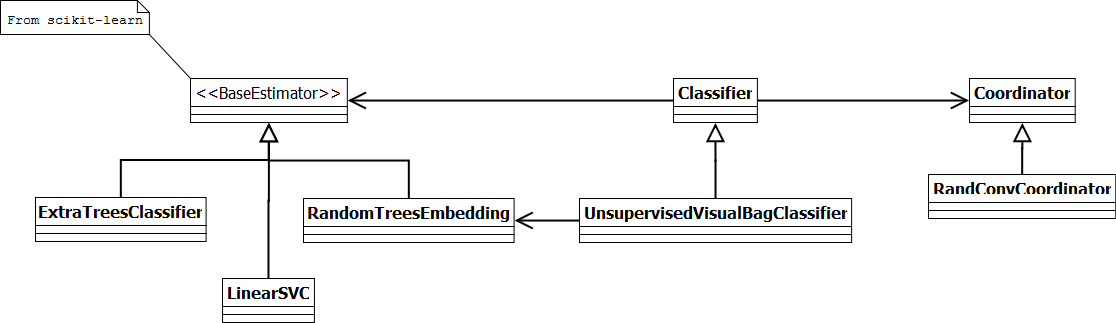
\includegraphics[width=1.00\textwidth]{images/uml-classifier.png}
			\caption{UML representation of the \texttt{Classifier} class and its major components}
			\label{fig:uml-classifier}
		\end{figure}
		
		
		\paragraph{}
		We now go back to the \texttt{RandConvCoordinator}. Its responsibility is to transform the subwindows into feature vectors. It proceeds by subdividing the dataset to parallelize the transformation. Then, the \texttt{ConvolutionalExtractor} process each image. This entails filtering the image by each element of the \texttt{FiniteFilter} thanks to the \texttt{Convolver}, the applying all the spatial poolings contained in the \texttt{MultiPooler} and finally extracting several subwindows via the \texttt{MultiSWExtractor}. Once all this is done, each filtered and pooled subwindow is passed through the \texttt{Extractor} and reassembled to form a coherent learning submatrix.
		\par
		The \texttt{FiniteFilter} objects are containers for filters. They pre-generate a finite number of filters thanks to the \texttt{FilterGenerator}. We will come back to those in the next paragraph. If we are working with RGB images, we need to use either a \texttt{Finite3Filter} or a \texttt{Finite3SameFilter}. The former produces a different filter per color component while the latter uses the same filter on each color. Also, we need to use an appropriate \texttt{Convolver}, namely the \texttt{RGBConvolver}.
		\par
		The subwindow extraction is carried out by the \texttt{MultiSWExtractor} whose sole purpose is to keep track of the subwindows to extract to the set of filtered and pooled images belonging to the same original image. The actual subwindow generation and extraction are delegated to the \texttt{SubWindowExtractor}.
		\par
		The transformation from subwindows to feature vector is the responsibility of the \texttt{Extractor} instance. In this case, a \texttt{ImageLinearizationExtractor} object. However, other mechanism could be implemented.
		All this is summarized by the figure \ref{fig:uml-ConvolutionalExtractor}.
		
		
		\begin{figure}
			\centering
				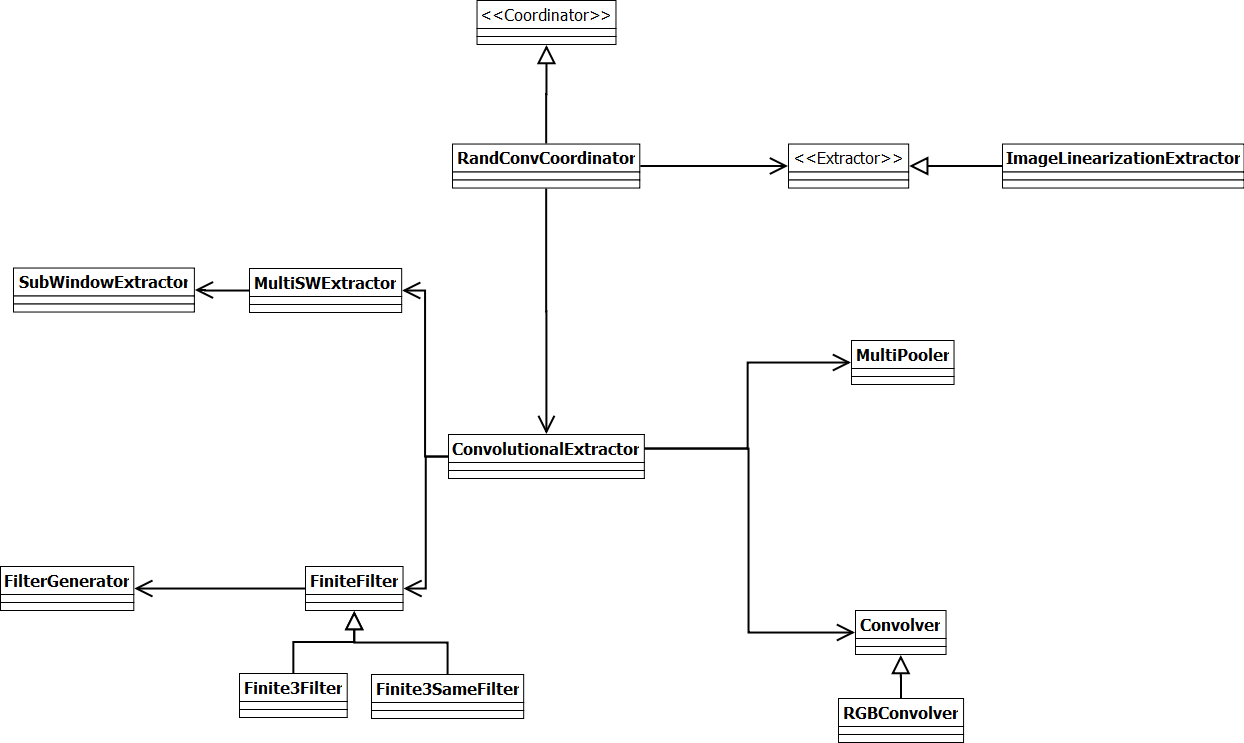
\includegraphics[width=1.00\textwidth]{images/uml-RandConvCoord.png}
			\caption{UML representation of the \texttt{RandConvCoordinator} and its major components}
			\label{fig:uml-ConvolutionalExtractor}
		\end{figure}
		

		
		
		\paragraph{}
		We now explore the \texttt{FilterGenerator}. They need two random number generators. One for drawing the values, either directly or not, and one for drawing the size. The base class is used for two of the generation methods : the discrete law generator and the zero-perturbation generator. The former is made by using a \texttt{CustomDiscreteNumberGenerator} while the later uses the base class of \texttt{NumberGenerator}. 
		As figure \ref{fig:uml-filtergen} displays, there is a class dedicated to each of the other generators.
		\par
		The \texttt{GaussianNumberGenerator} works by specifying a lower bound, an upper bound and the probability of being outside of that range. The \texttt{ClippedGaussianRNG} works similarly but in addition forces the values outside of the range to the appropriate bound.
		
		
		\begin{figure}
			\centering
				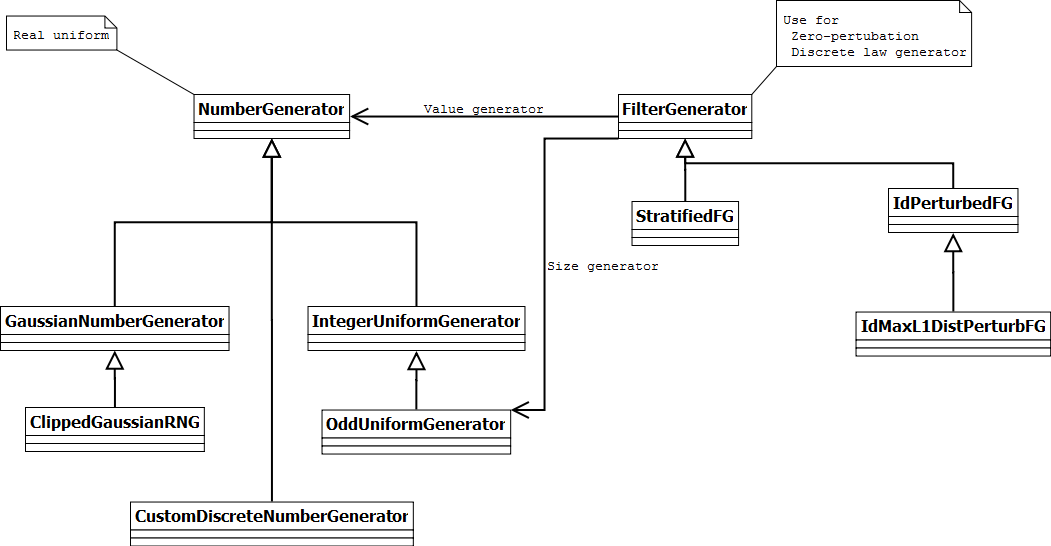
\includegraphics[width=1.00\textwidth]{images/uml-filtergen.png}
			\caption{UML representation of the \texttt{FilterGenerator}s and \texttt{NumberGenerator}s}
			\label{fig:uml-filtergen}
		\end{figure}
		
		
		\paragraph{}
		The \texttt{MultiPooler} class involved in the \texttt{RandConvCoordination} is a container of spatial poolings. As the figure \ref{fig:uml-pooling} depicts, our two groups of spatial poolings are presents.
		
		
		\begin{figure}
			\centering
				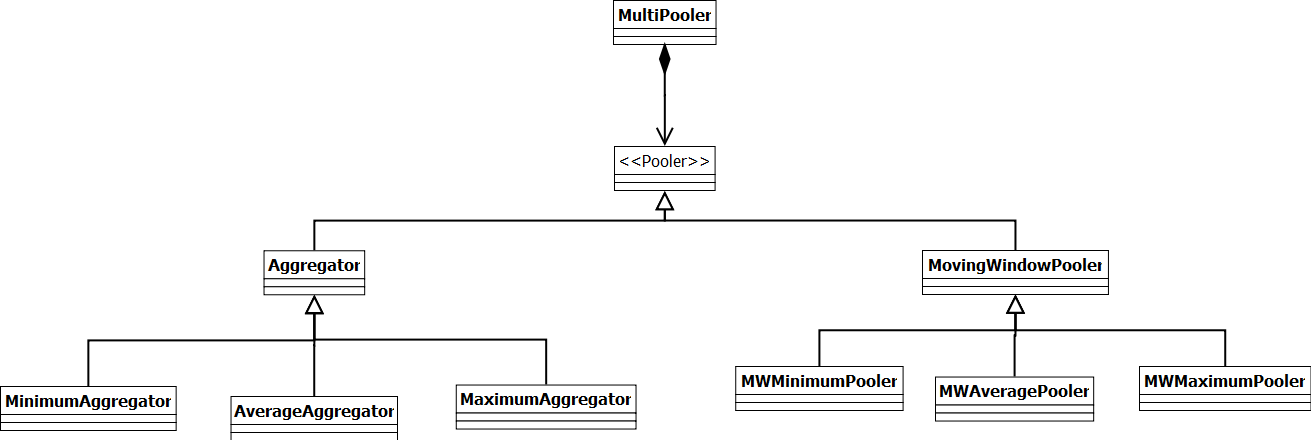
\includegraphics[width=1.00\textwidth]{images/uml-pooling.png}
			\caption{UML representaiton of the spatial poolings}
			\label{fig:uml-pooling}
		\end{figure}
		
		
		
		
		
		\subsection{Technical issues}
		The main limitation we will face is memory. The ExtraTrees implementation require 32-bits floats and the SVM, 64-bits floats. However, in the case of the ET-FL, the matrix is mostly sparse on therefore the 64-bits floats requirement of the SVM will not be troublesome. Thus, the space cost bottleneck is the input of the ExtraTrees, which require to hold all the data in memory. Considering 100 filters, 1 spatial pooling, subwindows resized in 16x16, 3 colors, 10 subwindows and the whole learning set (50,000 images) the RandConv method will produce 153.6 GB of data. For 39 filters (the custom filters plus the original image) and 20 subwindows with 9 spatial poolings (the configuration of the best results of \cite{}), 1,1 Tb would be required. Since we are limited to 288 GB, we will not be able to reproduce such a configuration.
		\par
		One way of sidestepping this limitation is to build several forests with a different subset of the features, a variant which might be called ``global random subset'' (GRS) of features. 
		In the case of the RandConv this can easily be done by choosing a subset of filters for each forest.
		
		\paragraph{}
		To a lesser extend, the time complexity will be an hindrance. It will not actually prevent any computation but we will have to plan carefully the experiment to carry out. For instance, our first example, which produces 153.6 GB of data, takes between 5h and 12h depending on the machine load.
		
	\section{Hyper-parameters summary}
	Before elaborating on the results, we will rapidly summarize all the hyper-parameters involved with the RandConv framework.
	
	\begin{itemize}
	
		\item Filter generation
		\begin{itemize}
			\item Size range
			\item Whether or not to produce squared filters
			\item Value range
			\item Filter generator
			\item Random law
			\item Other filter generator specific parameters (maximum distance, number of subdivisions,...)
			\item Filter normalization
			\item whether or not to include the original image
		\end{itemize}
		
		\item Spatial poolings
		\begin{itemize}
			\item Number and type of poolings
			\begin{itemize}
				\item Aggregation or moving window
				\item Pooling function : identity, minimum, average or maximum
			\end{itemize}
			\item Size of the neighborhood
		\end{itemize}
		
		\item Subwindow extraction
		\begin{itemize}
			\item Number of subwindows
			\item Subwindows cropping size
			\item Subwindows rescaling size
			\item Subwindows rescaling interpolation
		\end{itemize}
		
		\item ExtraTrees
		\begin{itemize}
			\item Number of trees (default : 10)
			\item Number of features of the local random subspace : $k$ (default : square root of the total number of features)
			\item Maximum depth (default : no maximum depth)
			\item Minimum sample to split : $n_{min}$ (default : 2)
			\item Minimum sample per leaf (default: 1)
			\item Whether or not to use bootstrap (default : no bootstrap)
		\end{itemize}
	\end{itemize}
	
	As we can see, the number of hyper-parameters is already large. We can divide them in two categories. On the one hand, we have structural parameters and on the other, traditional hyper-parameters. Structural parameters have a more profound impact than traditional ones. The filter generator and its random law and the number and type of spatial poolings form the structural parameters. Conceptually at least, changing one of them is closer to changing the classification method than only one of its hyper-parameters.
	\paragraph{}
	Three of the ExtraTrees hyper-parameters are used to control the pruning : the maximum depth, the minimum sample split and the minimum sample per leaf. The difference between the last two is that the first one does not attempt to split a node whose number of samples are under the given threshold, while the second does the split but rollback if any of the children are under the threshold. 
	\paragraph{}
	Several of the parameters can be fixed. The value range of the filters will be set as in the filter generator descriptions. Considering the size of the images, we will mostly focus on 3x3 to 9x9 filters. Since we are working with trees, we will use no normalization of the filters. Concerning the spatial poolings, we will also restrict ourselves to small neighborhoods. For comparative purposes, we will resize subwindows to have sizes of 16x16 with nearest neighbor interpolation, as in \cite{}. Moreover, we will extract subwindows of 24x24 to 32x32 pixels. For the ET-DIC variant, we will use the default trees parameters, which means no pruning. We will also use 30 trees (one per core). However, in the ET-FL approach, we will have to prune the trees and use more of them. The $n_{min}$ parameter will be set to 500 with 750 trees. Table \ref{tab:DefaultValuesForHyperParameters} displays the fix or default values of the hyper-parameters. Unless stated otherwise, these values are to be assumed in the next chapter.
	
	\begin{table}
		\centering
			\begin{tabular}{l|l}
			\hline
			Hyper-parameter & default value \\
			\hline
			Filter sizes & 3 to 9, both included\\
			Square sizes & True \\
			Filter value range & [-1, 1] \\
			Filter generator & \texttt{FilterGenerator} (Zero-perturbed generator)\\
			Random law & Real uniform\\
			Filter normalization & None\\
			Include original image & True\\
			Number of spatial poolings & 1 \\
			Type of spatial poolings & Average moving window \\
			Size of the neigborhood & 3x3 (moving window), 2x2 (aggregation)\\
			Number of subwindows & 10 \\
			Cropping size & 24x24 to 32x32 \\
			Rescaling size & 16x16 \\
			Interpolation & Nearest neighbor \\
			Number of trees & 30 (ET-DIC), 750 (ET-FL) \\
			$k$ & Square root of the total number of features \\
			Maximum depth & None \\
			Minimum sample to split & 2 (ET-DIC), 500 (ET-FL) \\
			Minimum sample per leaf & 1 \\
			Bootstrap & False \\
			\hline
			\end{tabular}
		\caption{Default values for hyper-parameters}
		\label{tab:DefaultValuesForHyperParameters}
	\end{table}
		
%TODO : feature evaluation --> by filter

		
\chapter{Result analysis}
In this chapter, we describe the experiments conducted with our new classification method and analyze their results. The chapter is divided into two sections. The first one tackles the direct classification scheme (ET-DIC), where the forest of extremely randomized trees serves as classificator. The second section describes the other variant where the extremely randomized trees are used to create a visual dictionary (ET-FL), while the actual classification is undergone by a support vector machine.
\par
We will use the following abbreviations :
\begin{itemize}
	\item \texttt{rc} : The \textbf{R}and\textbf{C}onv methods without the use of the original image.
	\item \texttt{rci} : The \textbf{R}and\textbf{C}onv methods with the use of the original \textbf{i}mage. As if the first filter were the identity filter.
	\item \texttt{pixit} : The method of \cite{}, where there is no filtering or pooling. Only the subwindows extraction
\end{itemize}
When the hyper-parameters value are not explicit, the default values are to be assumed (table \ref{tab:DefaultValuesForHyperParameters} of page \pageref{tab:DefaultValuesForHyperParameters}).
%describe the succession of experiment
	\section{Direct classification scheme}
	
		\subsection{Accuracy as a function of the learning set size}
		Our first experiment will be to measure how the accuracies of the different methods evolve as a function of the learning set size. We will test the \texttt{rci} method with both types of pooling mechanisms (aggregation and moving window). The aggregation pooling uses a neighborhood of 2x2 while the moving windows are of size 3x3. Both poolings uses an averaging function. We will limit ourselves to the zero-perturbed filter generator for now. In both cases, the same 100 filter are drawn. The 10 extracted subwindows are resized to 16x16. Consequently there are $(16 \times 16 \times 100 \text{ filters} \times 1 \text{ pooling})\times 3 \text{ colors} = 76,800$ features. The accuracy is measured on the whole testing set composed of 10,000 images. The\texttt{pixit} method will serve as reference.
		\paragraph{}
		We measure the accuracy for the learning set sizes of 500, 5,000, 10,000, 20,000, 30,000, 40,000 and 50,000. The result of this experiment is depicted by figure \ref{fig:accFLSsize}. The conclusion is clear : the aggregation pooling mechanism is not working (0.38 of accuracy). Although being of the smallest interesting size, the non-overlapping neighborhood windows already lose too much of the information. One might argue that using 3x3 moving subwindows allow for that variant to capture more of the spatial structure than 2x2 neighborhood. However, this does not seem to be the case as using 3x3 neighborhoods yields a lower accuracy of 0.35 for the whole learning set. Therefore, the bad performances of the aggregation mechanism must indeed comes from its abusive spatial compression. This is unfortunate because those poolings suffered less from the rescaling of the extracted subwindows. Considering the gap of accuracy between both methods, the following experiments will focus on the moving window poolings.
		\par
		Other observations are worth mentioning. Firstly, the ``good'' RandConv method performs well. It is consistently better than the \texttt{pixit}, although the difference might not be worth the trouble. The RandConv methods takes several hours whereas the \texttt{pixit} requires a couple of minutes at most. 
		%Secondly, around 30,000 training images the accuracy rate slows down. This indicates that learning set is big enough to create models of the appropriate complexity.
		Secondly, the graph shows the impact of using only a subset of the data. This information is important in case of hyper-parameter optimization, for instance, where some of the data must be set aside as validation set.
		
		\begin{figure}
			\centering
				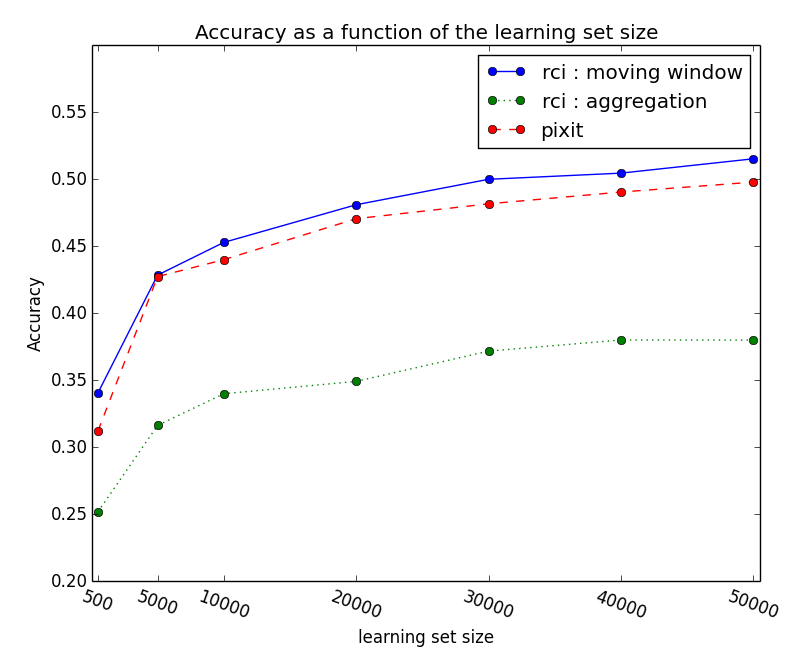
\includegraphics[width=1.0\textwidth]{images/accFLSsize.png}
			\caption{\label{fig:accFLSsize}Accuracy as a function of the learning set size (30 trees, $k=277$)}
		\end{figure}
		
		\paragraph{}
		Our best result so far is an accuracy of 0.515 due to the RandConv method with moving windows for spatial pooling. The \texttt{pixit} methods with the same parameters yields an accuracy of 0.50, while its best result is 0.53 for 20 subwindows, 10 trees and a minimum sample to split of 10. We will now analyze the variability of the method and how the method varies with some its hyper-parameters.
		%Validate small sized filters
		
		\subsection{\label{subsec:ETDICVariability}Variability}
		We now inspect the variability of the accuracy and of the filter importances. We will first look at the situation where the learning matrix is fixed and the variability can only come from the ExtraTrees. It is important to differentiate both types of variability. The one from the ExtraTrees would mainly be due to the high dimensionality of the problem. Indeed, the size of the local random subspace ($k = \sqrt{76,800} \simeq 277$) is relatively small compare to the total number of features : $\frac{277}{76,800} \simeq 3.6 \times 10^{-3}$. Therefore, different trees will end up making different choices. This is, of course, exactly the behavior we are looking for. However, with as few trees as 30, we may expect that different forests will have a high variability on the filter importances and consequently on the accuracy.
		\par
		We have run the ExtraTrees 12 times with the same hyper-parameters and the same learning matrix. Table \ref{AccVarTrees} holds the accuracies and table \ref{CorrMatFiltTreeVar} holds the first line of the correlation matrix of the filter importances between the tests. Figure \ref{FIVarTree} depicts the filter importances for the two firsts tests. The test number 0 corresponds to the results given in the previous section. As we can see, the variability is very small. More tests would be needed to establish a rigorous confidence interval but the conclusion seems clear nonetheless : ExtraTrees variability has no impact on the accuracy. This is also backed up by the evident stability of the filter importances. Such stability is due to the smoothing effect of aggregating all the feature importances of a given filter. The overall conclusion is that tree variability has no impact of the method for a given learning matrix. This stability also suggests that hyper-parameters such as the size of the local random subspace ($k$) and the number of trees will play little role to improving the accuracy. We will confirm that with the following experiments. The number of subwindows might, however, have more influence of the accuracy. This will also be established by one of the experiments.
		\par
		Let us digress on the filter importances. From figure \ref{FIVarTree}, we can see that several filters have a high importance ; of the same order of magnitude than the original image (filter 0). On the other hand, some filters bring little to none information in the classification process. Either these filters are not (co-)useful or the trees are to small to incorporate their usefulness. In regard to the correlations between tests, however, the co-uselfulness and complexity hypotheses are less likely. If it were one of these problems, the low-rated filters would have developed on different trees and therefore the filter importance profiles would be less similar. Therefore, the most likely hypothesis is that those filters are simply not useful. Inspecting them in parallel of the best ones might reveal information about the classification task. In any case, removing them to make room for more interesting filters can only improve accuracy. Sadly, the gain is unlikely to be substantial. Indeed, the current accuracy gain compare to the \texttt{pixit} is marginal, even though we already have many filters whose importance rivals the original image.
		
		
		\begin{table}
			\centering
			\begin{subtable}{0.5\textwidth}
				\begin{tabular}{c|c}
				\hline
				Test number & Accuracy \\
				\hline \hline
				0 & 0.5151 \\
				1 & 0.5119 \\
				2 & 0.5118 \\
				3 & 0.5136 \\
				4 & 0.5135 \\
				5 & 0.5141 \\
				6 & 0.5154 \\
				7 & 0.5114 \\
				8 & 0.5145 \\
				9 & 0.5156 \\
				10 & 0.5148 \\
				11 & 0.5118 \\
				\hline
				\end{tabular}
				\caption{\label{tab:AccVarTrees}Accuracy variability}
			\end{subtable}%
			\begin{subtable}{0.5\textwidth}
				\begin{tabular}{c|c}
				\hline
				Test number & Correlation with test 0\\
				\hline \hline
				0 & 1\\
				1 & 0.998 \\
				2 & 0.997 \\
				3 & 0.999 \\
				4 & 0.997 \\
				5 & 0.998 \\
				6 & 0.998 \\
				7 & 0.998 \\
				8 & 0.997 \\
				9 & 0.998 \\
				10 & 0.998 \\
				11 & 0.997 \\
				\hline
				\end{tabular}
				\caption{\label{tab:CorrMatFiltTreeVar}Correlation vector of the filter importances with test number 0}
			\end{subtable}
			\caption{\label{tab:TreeVar}Variability induced by the tree growing algorithm (same learning matrix)}
		\end{table}
		
		\begin{figure}
			\begin{subfigure}{.5\textwidth}
				\centering
				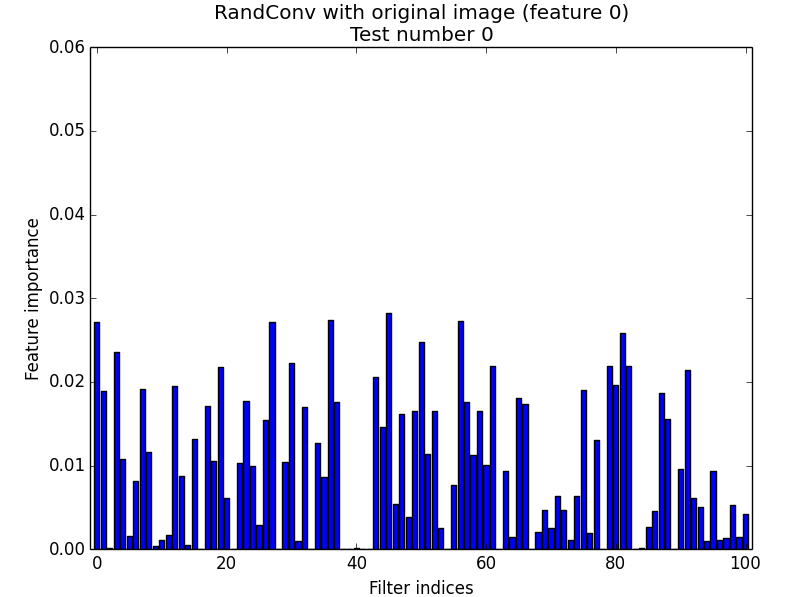
\includegraphics[width=1.\linewidth]{images/FIVarTree0.png}
				\caption{\label{fig:FIVarTree0}Test 0}
			\end{subfigure}%
			\begin{subfigure}{.5\textwidth}
				\centering
				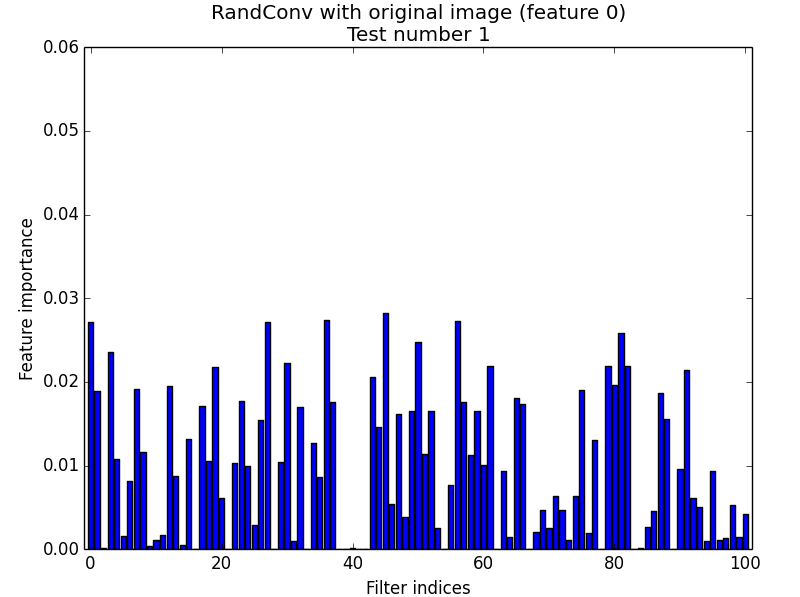
\includegraphics[width=1.\linewidth]{images/FIVarTree1.png}
				\caption{\label{fig:FIVarTree1}Test 1}
			\end{subfigure}
			\caption{\label{fig:FIVarTree}Filter importances for two different forests with the same parameters}			
		\end{figure}
		
		\paragraph{}
		We now turn to the variability produced by the RandConv with the other parameters fixed to their default values. There are three sources of variability :
		
		\begin{itemize}
			\item The filter generated
			\item The subwindows extracted
			\item The trees built
		\end{itemize}
		
		As we have just seen, the last source of variability is negligible, therefore, we will mainly assess the first two ones. We ran 10 more tests whose accuracies are shown in table \ref{tab:VarZeropertAcc}. Test 0 corresponds to our previous test. Once again, more tests would be required to establish a proper confidence interval but the variability, although more important than previously, seems to be quite low. Tests number 0 and number 1 are particularly good. Nevertheless, this has to be put in perspective : such low range of accuracies, although always welcome for a practical application, is not really significant in our context.
		\par
		Since we are using different filters, the importance profiles will be different from one another. Figure \ref{fig:FIGVar} illustrates this for the tests number 1, 5, 6 and 10. We expect the ideal situation to be when all the filters have the roughly same importances. Nevertheless, how the filter importances the accuracy in other circumstances is unclear and cannot be determined from the importance profile. This is made clearer by comparing the cumulative importances of several tests. Figure \ref{fig:FIGVarCumHist} depicts the situation for tests number 0, 1 and 6. For the 30 most influential filters, test 6 is between the other two curves, therefore we cannot predict anything about the accuracy. After that point, test 6 depicts a greater cumulative filter importance. This situation also implies that there are more lowly important filter in test 6 than test 0 or 1. Once again, we cannot deduce anything from it because test 1 is also greater than test 0 in term of both the cumulative filter importance and accuracy. Besides, the cumulative profile of test 5 is nearly identical to the one of test 0. Therefore, it is impossible to assess finely the accuracy from the importance profile.
		
		
		\begin{table}
			\centering
				\begin{tabular}{l|l}
				\hline
				Test number & Accuracy \\
				\hline \hline
				0 & 0.5151 \\
				1 & 0.5183 \\
				2 & 0.5117 \\
				3 & 0.5137 \\
				4 & 0.5095 \\
				5 & 0.5094 \\
				6 & 0.5093 \\
				7 & 0.5117 \\
				8 & 0.5129 \\
				9 & 0.5116 \\
				10 & 0.5124 \\
				\hline
				\end{tabular}
			\caption{\label{tab:VarZeropertAcc}Accuracy of several tests}
		\end{table}
		
		
		\begin{figure}
			\begin{subfigure}{.5\textwidth}
				\centering
				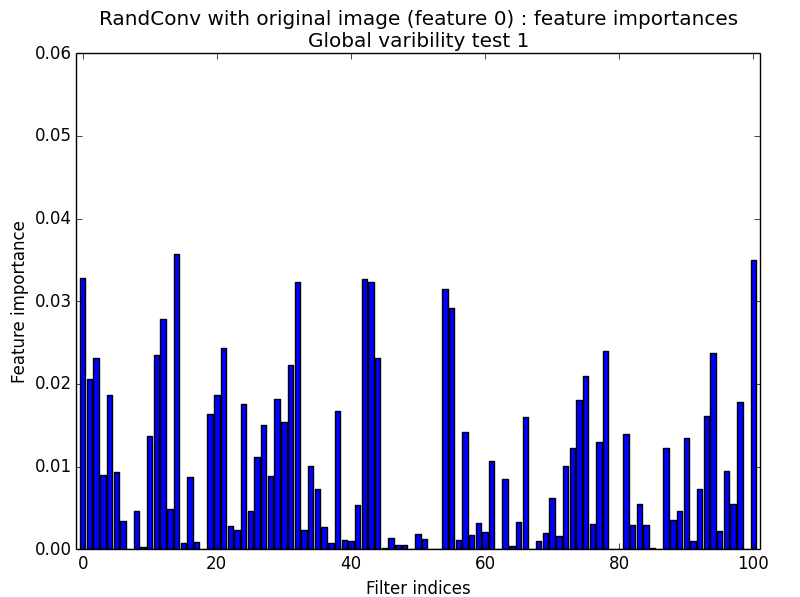
\includegraphics[width=1.\linewidth]{images/FIGVar1.png}
				\caption{\label{fig:FIGVar1}}
			\end{subfigure}%
			\begin{subfigure}{.5\textwidth}
				\centering
				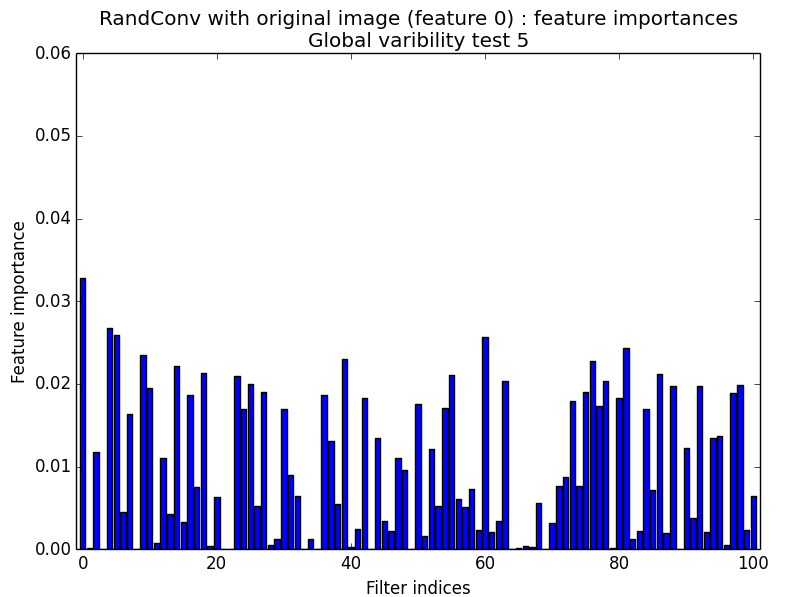
\includegraphics[width=1.\linewidth]{images/FIGVar5.png}
				\caption{\label{fig:FIGVar5}}
			\end{subfigure}
			\begin{subfigure}{.5\textwidth}
				\centering
				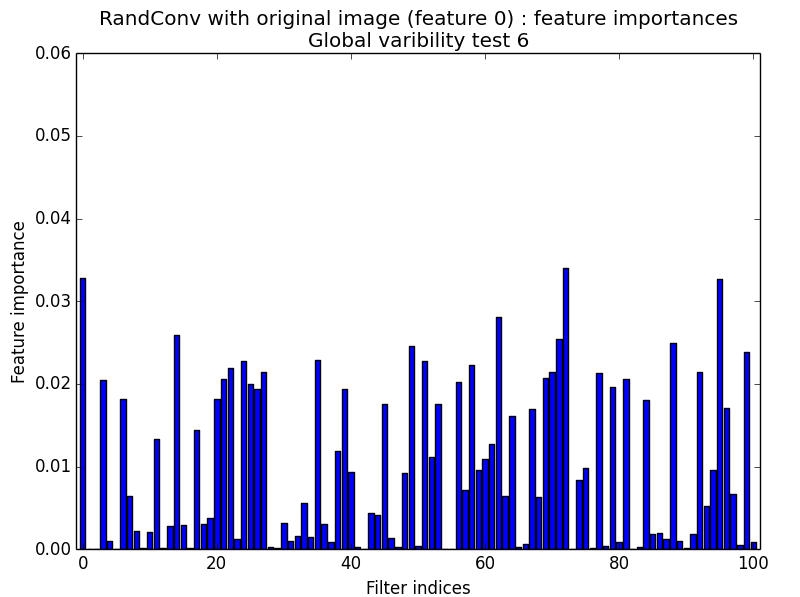
\includegraphics[width=1.\linewidth]{images/FIGVar6.png}
				\caption{\label{fig:FIGVar6}}
			\end{subfigure}%
			\begin{subfigure}{.5\textwidth}
				\centering
				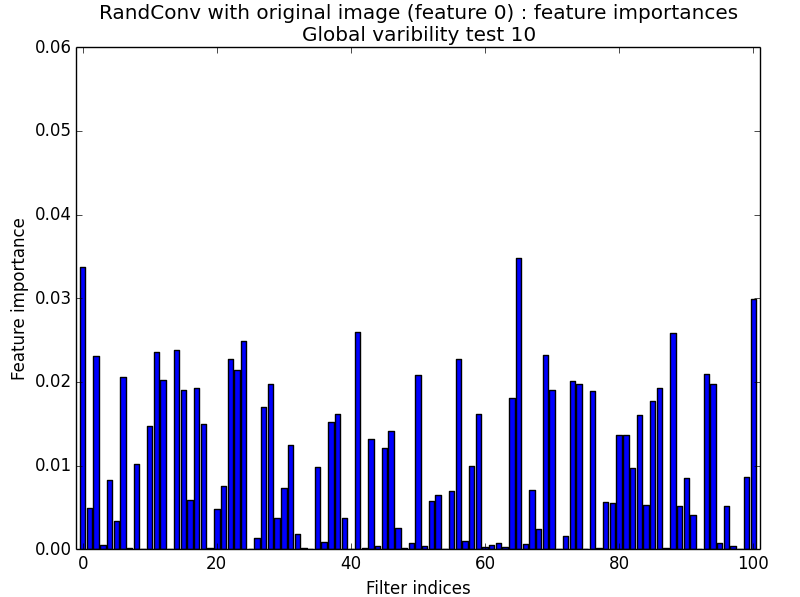
\includegraphics[width=1.\linewidth]{images/FIGVar10.png}
				\caption{\label{fig:FIGVar10}}
			\end{subfigure}
			\caption{\label{fig:FIGVar}Filter importances with global variability}
		\end{figure}
		
		\begin{figure}
			\centering
				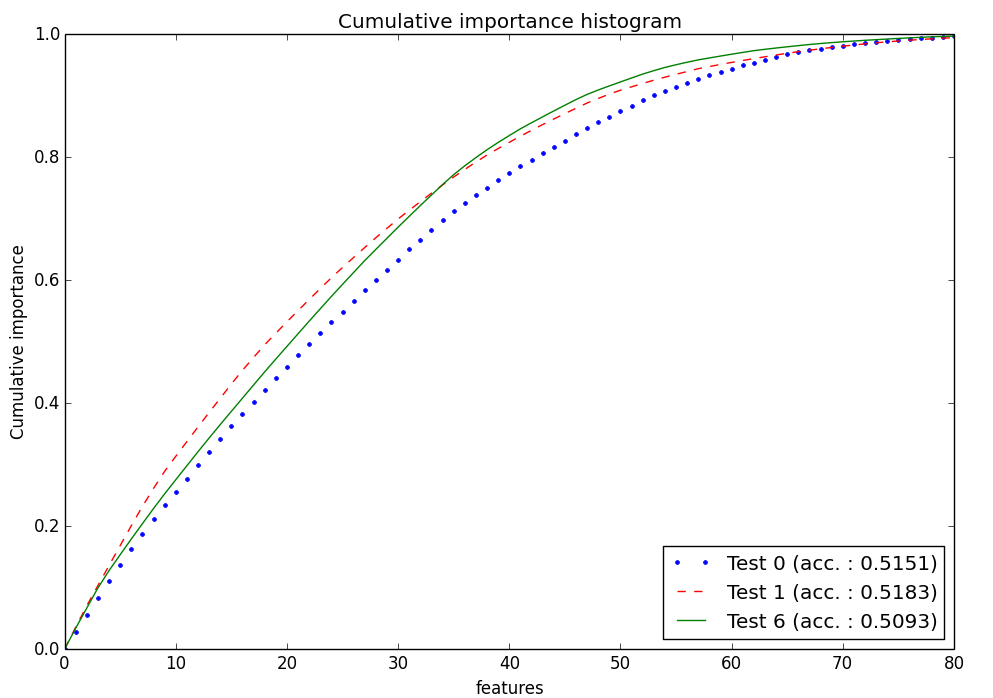
\includegraphics[width=1.0\textwidth]{images/FIGVarCumHist.png}
			\caption{\label{fig:FIGVarCumHist}Cumulative filter importance (first 80 filters)}
		\end{figure}
		
		\paragraph{}
		So far, we have learned that the RandConv method was surprisingly stable. Fortunately, this will allow us to draw conclusions from few experiments, a welcome surprise considering their running time. We will now inspect further the influence hyper-parameters with a same set of filters if not a same learning matrix.
		
		\subsection{Influence of the number of subwindows}
		As a reminder, the number of subwindows enlarges the learning set and therefore allows for more complex models. In this experiment, we tested how accuracy varied with the number of extracted subwindows. We used 1, 5, 10 and 14 subwindows. The memory limited us to that threshold in order to keep the other parameters to their default values (table \ref{DefaultValuesForHyperParameters}, page \pageref{DefaultValuesForHyperParameters}). We also tested the method where no subwindows are extracted but rather the whole image is used directly. The results are reported at table \ref{AccFNbSW}. The filters were the same in all the tests.
		\par
		As we might have suspected, using the whole image yields better accuracy than using only one random subwindows. However, a few of them already accounts for a better accuracy. Judging by the accuracy jump between 5 and 10 subwindows compare to the stagnation between 10 and 14 subwindows, we may conclude that 10 subwindows allows for complex-enough models. 
		
		\begin{table}
			\centering
				\begin{tabular}{l|l}
				\hline
				Number of subwindows & Accuracy \\
				\hline \hline
				1 (whole image) & 0.44\\
				1 (subwindow) & 0.40 \\
				5 & 0.48 \\
				10 & 0.515 \\
				14 &  0.514\\
				18 &  0.521 \\
				\hline
				
				\end{tabular}
			\caption{\label{tab:AccFNbSW}Accuracy as a function of the number of subwindows}
		\end{table}
		
		
		\subsection{Influence of the number of trees}
		The accuracy is usually an increasing function of the number of trees. In this subsection, we will see how this function behaves for our method and we will look at the filter importances as well. In section \ref{subsec:ETDICVariability} about the variability, we foresaw that increasing the number of trees would have little influence on the filter importances. Now is the time to validate this thesis. Once again, the other parameters will be set to the default values of table \ref{tab:DefaultValuesForHyperParameters} on page \pageref{tab:DefaultValuesForHyperParameters} and the learning matrix is the same in all the tests. Consequently, the only source of variability is due to the forest creation.
		\paragraph{}
		In this experiment, we measure the accuracy for the following number of trees : 10, 30, 50, 100, 300 and 500. 
		
		%TODO : change accordingly
		The result of this experiment is depicted by figure \ref{fig:accFnbTrees}. As expected, we observe an increasing function of the number of trees. The local decreases are small and are due to the randomization of the tree growing algorithm. From a relatively low accuracy of 0.492 at 10 trees, the method quickly jumps to the value of 0.515 for 30 trees and then to 0.521 at 50 trees. The increase slows down a bit at 100 trees with an accuracy of 0.526. After that, the increase rate drops considerably. Two remarks are in order. Firstly, we observe the classical increasing pattern, which means that the number of trees can be chosen solely with respect to the allowable computational budget. However, for a given learning matrix, the accuracy is upper bounded, as we can see from the rate decrease. Secondly, the 30-trees accuracy is closer to the 500-trees' than to the 10-trees'. Adding our observation about variability, we may conclude that using 30 trees allow us a good assessment of the method characteristics. 
		\begin{figure}
			\centering
				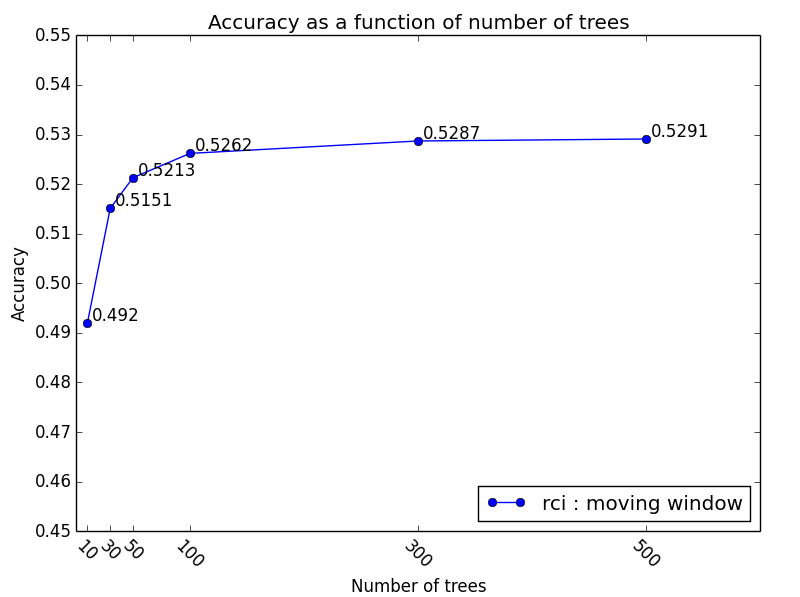
\includegraphics[width=1.0\textwidth]{images/accFnbTrees.png}
			\caption{\label{fig:accFnbTrees}Accuracy as a function of the number of trees}
		\end{figure}
		
		
		\par
		We now turn to the filter importances in the classification process. Table \ref{tab:CorrVecNbTrees} displays the filter importance correlation between the test with 10 trees and the other tests. As we had predicted, the number of trees does not impact the filter importances. Therefore, using 30 trees is well enough to assess filter usefulness as well.
		
		\begin{table}
			\centering
				\begin{tabular}{l|l}
				\hline
				Number of trees & Correlation \\
				\hline \hline
				10 & 1 \\
				30 & 0.996 \\
				50 & 0.998 \\
				100 & 0.998 \\
				300 & 0.998 \\
				500 & 0.998 \\
				\hline
				\end{tabular}
			\caption{\label{tab:CorrVecNbTrees}Filter importance correlation with 10 trees}
		\end{table}
		
		
		\subsection{Influence of the minimum number of samples to split}
		This parameter control the model complexity. In the previous experiments, the trees were fully grown ($n_{min} = 2$) and variability reduction was achieve through the smoothing effect of the forests prediction aggregation. Still, the model might be too complex to begin with, thus requiring some pruning. We tested the following values of this hyper-parameter : 2, 10, 50, 500. The corresponding accuracies are : 0.515, 0.512, 0.498, 0.453. Once again we see that the default value performs well. Besides, pruning too much the trees is harmful : the models are not complex enough any longer.
		\par
		The influence on the filter importances is more interesting. We clearly can identify two groups of filter. The first one is composed of the filters whose importance increases. This increase implies a decrease of the filter importances in the second group. It is thus possible to see where the filter is used in the trees. The first group holds the top of the tree. This was already obvious for the filters whose importance was either large or low. However, this approach sheds more light on the average filters, where we can observe divergent behaviors. Average filters of the second group are purely co-useful filters : they bring little information on their own but are helpful with the other filters. This characteristic resembles the ``V-structures'' of the graphical probabilistic models. On a specific classification task, these particular filters may be worth investigating. It might be difficult to identify the filters on which they depend, however.
		
	\subsection{Influence of the number of filters}
	Our expectation regarding the number of filters is that, with few of them, the accuracy might be better or worse than the \texttt{pixit}'s depending on the filter usefulnesses. With many filters, however, there should be enough usefulness altogether to be able to beat the \texttt{pixit} systematically. The accuracy should increase accordingly with the number of filters as long as the learning set size allows for complex-enough model. However, from the comment on the variability (subsection \ref{subsec:ETDICVariability}), we suspect that we will reach an upper bound quite fast. 
	\par
	From a more practical point of view, we will have to limit ourselves to 180 filters, which should not be a problem if we were right about the upper bound. Table \ref{tab:AccFNbFilt} presents the accuracies for 10, 38 (the number of filters in the custom generator),100, 120, 180 filters. As we can see, from 100 filters on, there is no accuracy gain and the filter and subwindow variabilities are responsible for the slight differences of accuracy. We would need a more profound analysis to determine whether or not the accuracy obtained with 38 filters is statically inferior to the 100 filter case's. In any case, it is closer to the accuracy of the 100 filters than of the 10 filters.
	
	\begin{table}
		\centering
			\begin{tabular}{l|l}
			\hline
			Number of filters & Accuracy \\
			\hline \hline
			10  & 0.4831 \\
			38 & 0.5087 \\
			100 & 0.5151 \\
			120 & 0.5112 \\
			180 & 0.5150 \\
			\hline
			\end{tabular}
		\caption{\label{tab:AccFNbFilt}Influence of the number of filters on the accuracy}
	\end{table}
	
		
	\subsection{Influence of the filter generator}
	%Compare rci to rc
	
	\subsection{Influence of spatial poolings}
	In this subsection, we tackle the influence of the spatial poolings with a couple of experiments. We will resort to the 39 custom filters so as to be able to use several poolings. The only source of randomness is the drawing of subwindows. The influence on the accuracy is summarized by table \ref{tab:AccFpoolings}. We can clearly see that the poolings have a beneficial effect on the accuracy, in particular the maximum. %test with maximal pooling on zeropert
	%rci_zeropert_120_filters no poolings : 0.4912
	Choosing the best pooling must either be done by cross-validation or not done : using several poolings should not reduce the accuracy dramatically. The main drawback of this last option is that the memory might be better used in another fashion. Using the same pooling at different spatial scales is may or may not be interesting.
	
	\begin{table}
		\centering
			\begin{tabular}{l|l}
			\hline
			Number of filters & Accuracy \\
			\hline \hline
			no pooling & 0.4816 \\
			3x3 minimum & 0.5151\\
			3x3 average & 0.5057 \\
			3x3 maximum & 0.5476 \\
			3x3 min., avg. max. & 0.5454 \\
			3x3, 5x5, 7x7 avg. & 0.5173 \\
			3x3, 5x5, 7x7 max. & 0.5741 \\
			\hline
			\end{tabular}
		\caption{\label{tab:AccFpoolings}Influence of the poolings on the accuracy with the custom filters}
	\end{table}
	
	\paragraph{}
	We now turn to the filter importances. Figure \ref{fig:FIPool} depicts the profiles for the single pooling cases. Some filters always have a high or low importance. For other filters, however, the importances vary. Concerning the profiles, if not the accuracies, the no pooling and average strategies are close, with a correlation of 0.954 (see the correlation matrix on table \ref{tab:FIPoolCorr}). The major difference comes from the number 20, which is a high pass filter. %Have a look at frequency response with and without the averaging
	The other pieces of information given by the correlation matrix are as one might expect.
	More interesting, we can observe that the profiles can be importantly influenced by the pooling, which means that it does bring information and increase some filter usefulnesses. In the occasion of filter 28 (the west compass gradient mask), the maximum pooling even goes as far as giving it more importance than other filters appreciated by the remaining poolings. 
	Interpreting the cumulative importance diagram (figure \ref{fig:FIPoolSeveral}) is, once more, complicated and we will limit ourselves to the following observation. The maximum pooling is the closet example to a straight line (the ideal situation where every filter has the same importance) we have seen so far and also scores the best accuracy for now. Despite the closeness of the no pooling strategy, however, it does not score a high accuracy.
	
	
	\begin{figure}
		\begin{subfigure}{.5\textwidth}
			\centering
			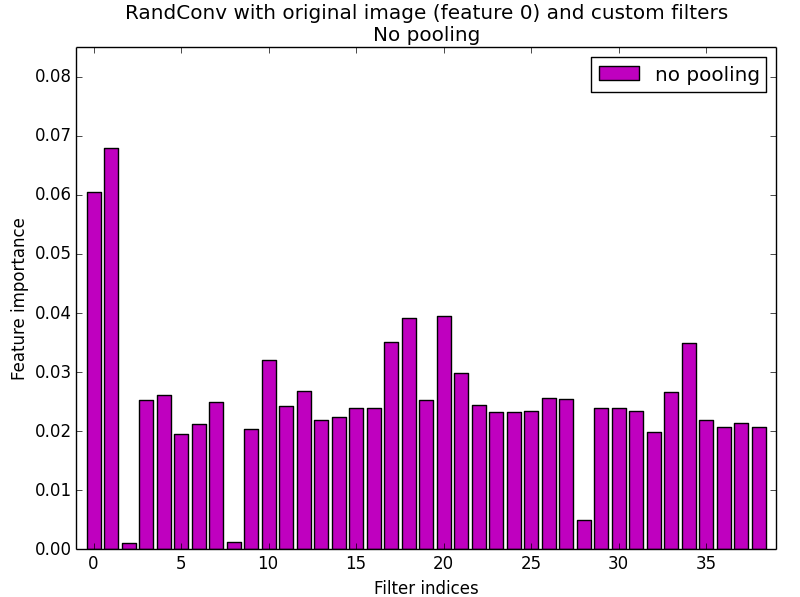
\includegraphics[width=1.\linewidth]{images/FIPoolNo.png}
			\caption{\label{fig:FIPoolNo}}
		\end{subfigure}%
		\begin{subfigure}{.5\textwidth}
			\centering
			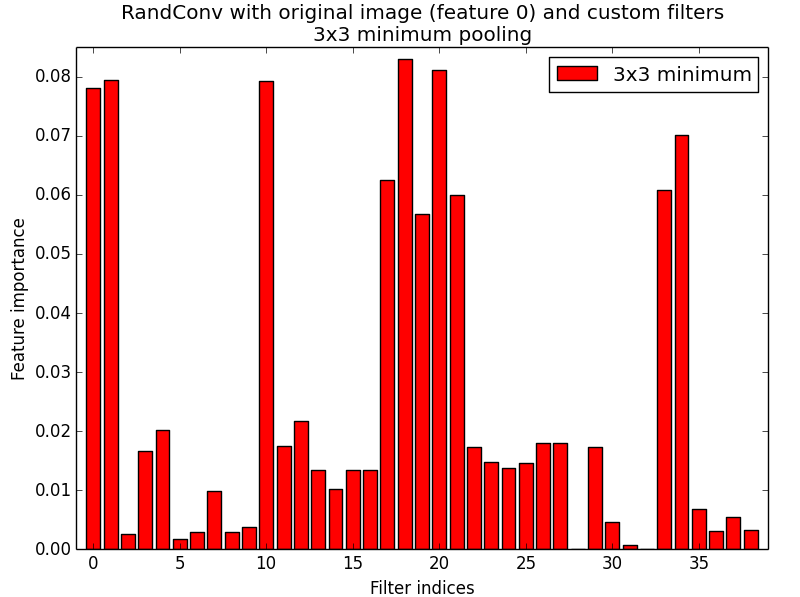
\includegraphics[width=1.\linewidth]{images/FIPoolMin.png}
			\caption{\label{fig:FIPoolMin}}
		\end{subfigure}
		\begin{subfigure}{.5\textwidth}
			\centering
			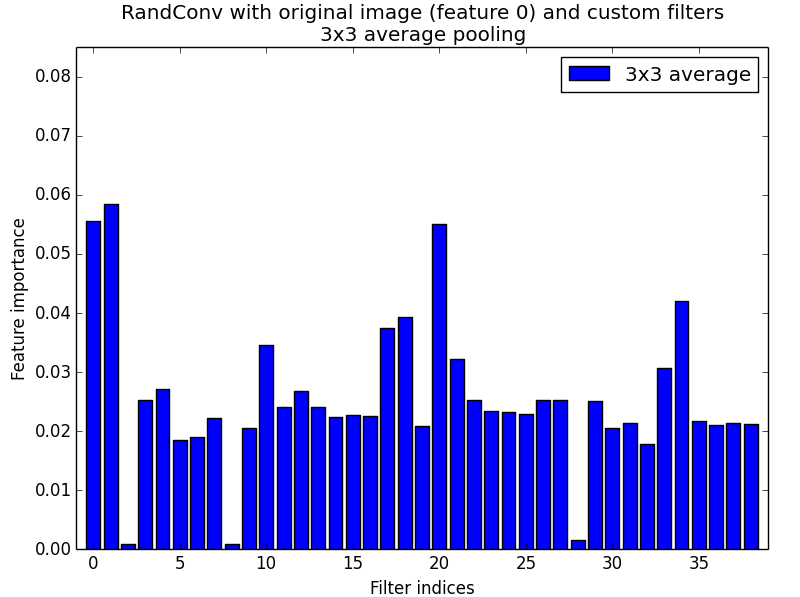
\includegraphics[width=1.\linewidth]{images/FIPoolAvg.png}
			\caption{\label{fig:FIPoolAvg}}
		\end{subfigure}%
		\begin{subfigure}{.5\textwidth}
			\centering
			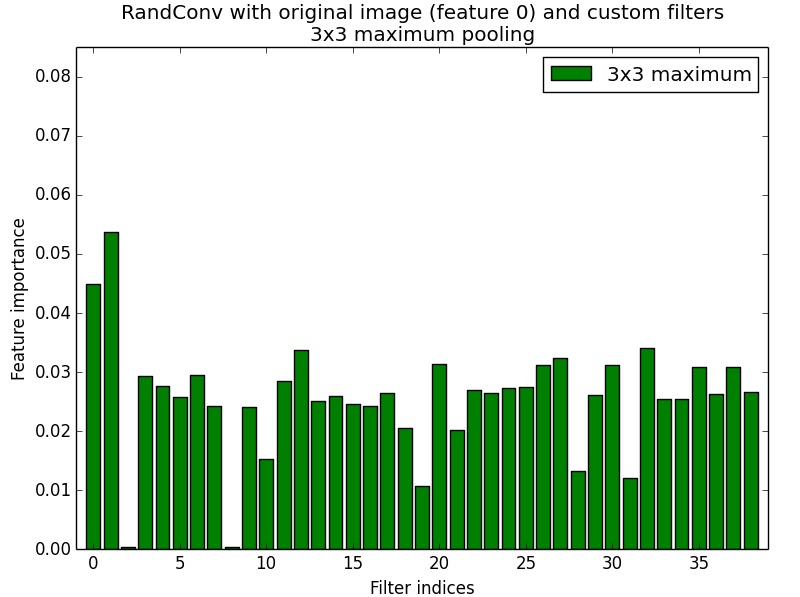
\includegraphics[width=1.\linewidth]{images/FIPoolMax.png}
			\caption{\label{fig:FIPoolMax}}
		\end{subfigure}
		\caption{\label{fig:FIPool}Filter importances with different types of poolings}
	\end{figure}
	
	
	\begin{table}
		\centering
			\begin{tabular}{|c||c|c|c|c|}
			\hline
			Pooling & no pooling & 3x3 minimum & 3x3 average & 3x3 maximum\\
			\hline \hline 
			no pooling & 1 & & &  \\
			\hline
			3x3 minimum & 0.762 & 1 & & \\
			\hline
			3x3 average & 0.954 & 0.826 & 1 & \\
			\hline
			3x3 maximum & 0.723 & 0.226 & 0.661 & 1 \\
			\hline
			\end{tabular}
		\caption{\label{tab:FIPoolCorr}Correlation matrix of the filter importances between the poolings}
	\end{table}
	
	
	\begin{figure}
		\centering
			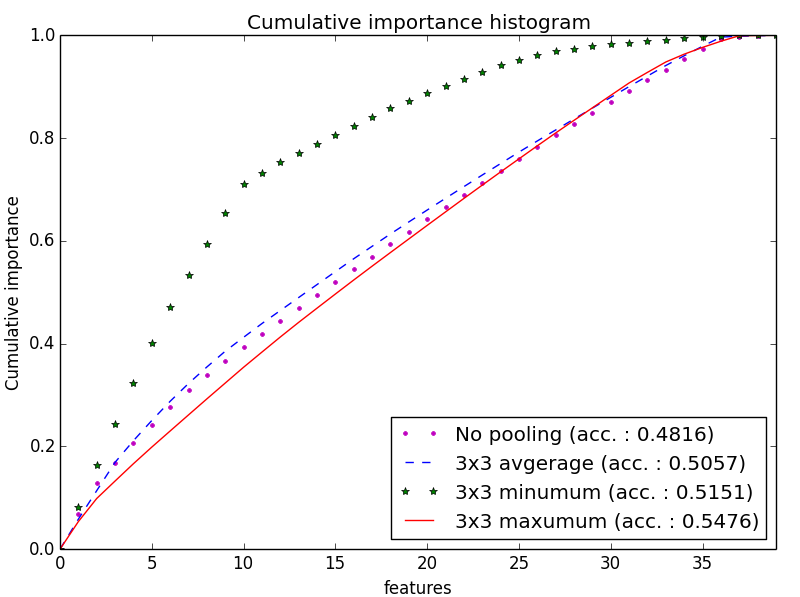
\includegraphics[width=1.0\textwidth]{images/FIPoolCumul.png}
		\caption{\label{fig:FIPoolCumul}Cumulative filter importances with different types of poolings}
	\end{figure}
	
	\par
	The observation of single pooling strategies bode well for their combine application. Yet, it may happen that they shade each other in a co-utilization scenario. In turns out this is a empty threat. The correlation between the corresponding importances are above 0.96 for all the pooling strategies (no pooling included). This is visually illustrated by figure \ref{fig:FIPoolNoAvgMinMax}. Each group of four bars belong to the same linear filter. 
	
	\begin{figure}
		\centering
			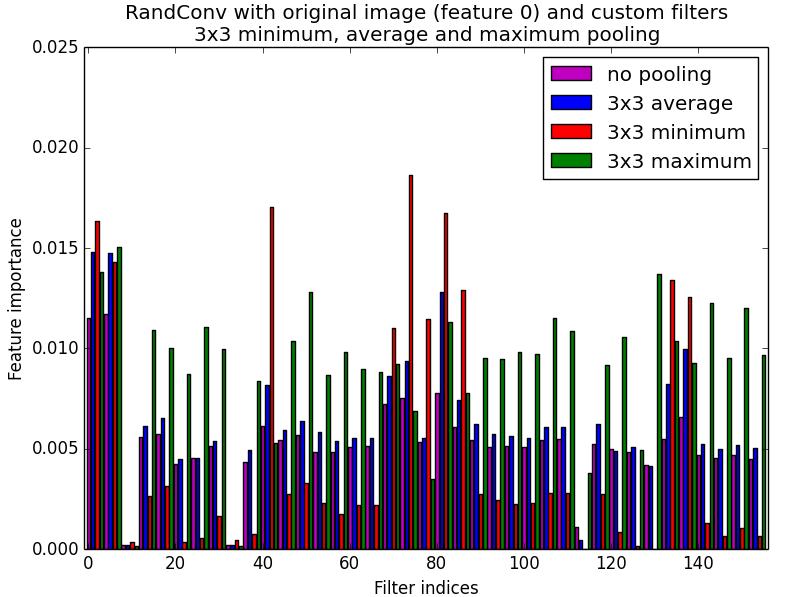
\includegraphics[width=1.0\textwidth]{images/FIPoolNoAvgMinMax.png}
		\caption{\label{fig:FIPoolNoAvgMinMax}Filter importances with several poolings}
	\end{figure}
	
	\par
	Figure \ref{fig:FIPoolScale} displays the filter profile for several poolings only differing by the moving window size. Most filters seems to favor larger windows. This (non-)locality preference is problem dependent.
	
	
	\begin{figure}
		\begin{subfigure}{.5\textwidth}
			\centering
			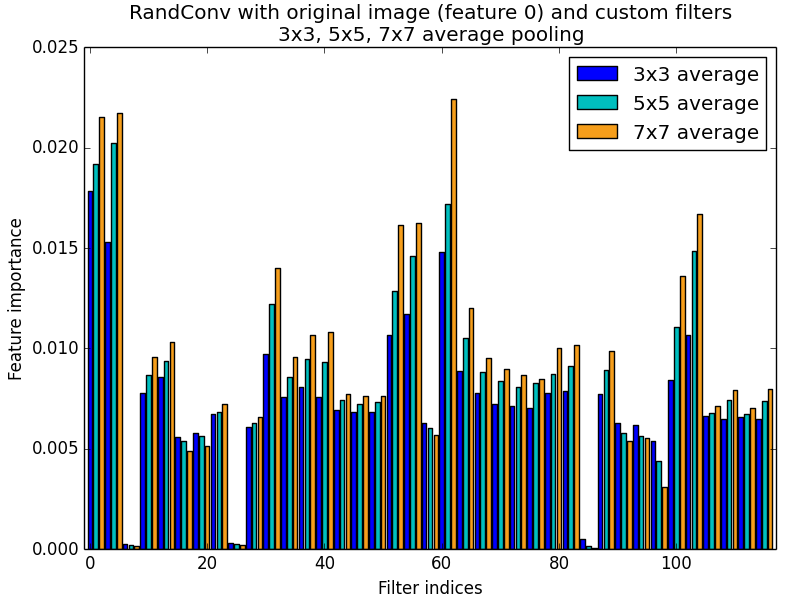
\includegraphics[width=1.\linewidth]{images/FIPoolAvg357.png}
			\caption{\label{fig:FIPoolAvg357}}
		\end{subfigure}%
		\begin{subfigure}{.5\textwidth}
			\centering
			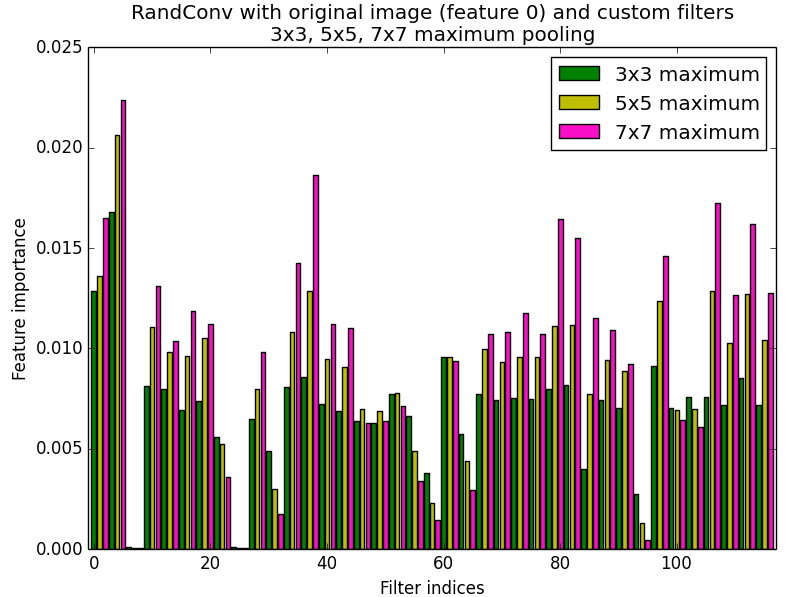
\includegraphics[width=1.\linewidth]{images/FIPoolMax357.png}
			\caption{\label{fig:FIPoolMax357}}
		\end{subfigure}
		\caption{\label{fig:FIPoolScale}Filter importances with several pooling scales}
	\end{figure}
		
	
	\paragraph{}
	Using a more appropriate spatial pooling is what has brought us the best improvement so far. Since poolings do not interfere with each other, an alternative to picking the best one is simply to use several. In doubt, a combination of the minimum and maximum pooling should do. If the best one is known, however, it might be worth investing the extra free memory to additional subwindows.
	

	%Fortunately, the default parameters works well --> No optimization bias
	\section{Feature learning scheme}
	The previous section focused on the ET-DIC pros and cons. We now turn to the ET-FL mode. In this mode, we use totally randomized trees to build a visual dictionary and the actual classification is carried out by a SVM. 
	\par
	This mode is less prone to a deep analysis of the influence of the hyper-parameters. The parameter $k$ is fixed to 1, and the number of subwindows, the number of trees and the minimum number of samples to split all influence the number of leaves in a well-understood fashion. An increase in the first two will produce an increase of the number of leaves and ultimately of the discriminant power. Therefore, the number of subwindows will be severely limited by the memory requirement while the number of trees limitation will be the computational time, although to a lesser extent. A good tradeoff must then be found between the number of subwindows and number of filters and spatial poolings. 
	Since we are not averaging the results any longer, we have lost the ability to reduce the model variability and must resort to pruning in order to limit its complexity. Usually, the optimal pruning should be obtained by cross-validation. However, for our database, a good value of $n_{min} = 500$ has already been established (\cite{}). 
	%describe the succession of experiment
	\subsection{Accuracy}
	
	
\chapter{Conclusion and perspective}
%less overlap than MW but more than aggreg
 
\bibliographystyle{apalike}
\bibliography{biblio}
  
\end{document}	


